% =============================================================================
%  Songdo Urban Digital Memory -- Project Handbook
%  Database Management and Practice (IBT3205-001), Inha University, Fall 2026
%
%  COMPILER: XeLaTeX.  On Overleaf: Menu -> Compiler -> XeLaTeX.
%  Locally:  xelatex main.tex  (run twice for the table of contents and references)
%
%  The file is self-contained: it uses only packages that ship with TeX Live.
%  Screenshots are read from outputs/evidence/screenshots/ when that folder is
%  present next to main.tex; otherwise a framed placeholder is printed instead,
%  so the document still compiles when main.tex is uploaded on its own.
%  Korean text uses the first Korean font found (Noto Serif CJK KR, UnBatang,
%  Malgun Gothic, NanumMyeongjo); without one it still compiles.
% =============================================================================
\documentclass[11pt,a4paper]{article}

% ---- engine check -----------------------------------------------------------
\usepackage{iftex}
\RequireXeTeX

% ---- fonts ------------------------------------------------------------------
\usepackage{fontspec}
\defaultfontfeatures{Ligatures=TeX}
\newif\ifkorean
\IfFontExistsTF{Noto Serif CJK KR}{\def\krfont{Noto Serif CJK KR}\koreantrue}{%
  \IfFontExistsTF{UnBatang}{\def\krfont{UnBatang}\koreantrue}{%
    \IfFontExistsTF{Malgun Gothic}{\def\krfont{Malgun Gothic}\koreantrue}{%
      \IfFontExistsTF{NanumMyeongjo}{\def\krfont{NanumMyeongjo}\koreantrue}{}}}}
\ifkorean
  \usepackage{xeCJK}
  \xeCJKsetup{CJKspace=true}
  \setCJKmainfont{\krfont}
  \setCJKsansfont{\krfont}
  \setCJKmonofont{\krfont}
\fi

% ---- layout -----------------------------------------------------------------
\usepackage[a4paper,margin=2.3cm,headheight=14pt]{geometry}
\usepackage{microtype}
\usepackage[dvipsnames,table]{xcolor}
\usepackage{graphicx}
\usepackage{array,booktabs,tabularx,xltabular}
\usepackage{enumitem}
\usepackage{fancyhdr}
\usepackage{titlesec}
\usepackage{caption}
\usepackage{needspace}
\usepackage[most]{tcolorbox}
\usepackage{listings}
\usepackage{tikz}
\usetikzlibrary{positioning,arrows.meta,shapes.geometric,fit,calc}
\usepackage[obeyspaces,spaces]{url}
\usepackage[colorlinks=true,linkcolor=NavyBlue,urlcolor=NavyBlue,citecolor=NavyBlue,
            pdftitle={Songdo Urban Digital Memory - Project Handbook},
            pdfauthor={Songdo Urban Digital Memory team}]{hyperref}

% ---- values to fill in ------------------------------------------------------
% The live demo URL from Render (Service -> Settings).  Leave as is if not deployed.
\newcommand{\LiveURL}{https://songdo-urban-memory.onrender.com}
\newcommand{\RepoURL}{https://github.com/Islamchik26/Songdo-Urban-Digital-Memory}
\newcommand{\TeamName}{Songdo Urban Digital Memory team}
\newcommand{\HandbookDate}{November 2026}
\newcommand{\shotdir}{outputs/evidence/screenshots}

% ---- colours and styles -----------------------------------------------------
\definecolor{inha}{HTML}{0B3D91}
\definecolor{accent}{HTML}{0F7B6C}
\definecolor{codebg}{HTML}{F5F7FA}
\definecolor{rule}{HTML}{C9D1DC}
\definecolor{passg}{HTML}{1E7B34}
\definecolor{limo}{HTML}{A15C00}

\setlength{\parindent}{0pt}
\setlength{\parskip}{0.55em}
\renewcommand{\arraystretch}{1.18}
\setlist{itemsep=0.15em,topsep=0.3em}

\titleformat{\section}{\Large\bfseries\color{inha}}{\thesection}{0.7em}{}[{\color{rule}\titlerule}]
\titleformat{\subsection}{\large\bfseries\color{inha}}{\thesubsection}{0.6em}{}
\titleformat{\subsubsection}{\normalsize\bfseries}{\thesubsubsection}{0.5em}{}
\titlespacing*{\section}{0pt}{1.4em}{0.8em}

\pagestyle{fancy}
\fancyhf{}
\fancyhead[L]{\small\color{gray}Songdo Urban Digital Memory}
\fancyhead[R]{\small\color{gray}Project Handbook}
\fancyfoot[C]{\small\thepage}
\renewcommand{\headrulewidth}{0.3pt}

\captionsetup{font=small,labelfont={bf,color=inha},skip=6pt}

% identifiers in running text: typewriter, may break after . _ /
\DeclareUrlCommand\code{\urlstyle{tt}}
% snippets with spaces: typewriter text that keeps its spaces (breaks only at spaces)
\newcommand{\cmd}[1]{\texttt{\detokenize{#1}}}
\def\UrlBreaks{\do\.\do\_\do\/\do\-\do\,}

\newcommand{\pass}{\textcolor{passg}{\textbf{PASS}}}
\newcommand{\limited}{\textcolor{limo}{\textbf{LIMITED}}}
\newcommand{\ra}{\ensuremath{\rightarrow}}
% defense question and answer
\newcommand{\qa}[2]{\par\needspace{4\baselineskip}%
  {\bfseries\color{inha}Q.\ #1\par}\nopagebreak\smallskip #2\par\medskip}

\newtcolorbox{keybox}[1][]{enhanced,breakable,colback=inha!4,colframe=inha!70,
  boxrule=0.6pt,arc=2pt,left=8pt,right=8pt,top=6pt,bottom=6pt,
  fonttitle=\bfseries,title={#1}}
\newtcolorbox{notebox}[1][]{enhanced,breakable,colback=accent!5,colframe=accent!70,
  boxrule=0.6pt,arc=2pt,left=8pt,right=8pt,top=6pt,bottom=6pt,
  fonttitle=\bfseries,title={#1}}

\lstdefinestyle{base}{
  basicstyle=\ttfamily\footnotesize,
  backgroundcolor=\color{codebg},
  frame=single, rulecolor=\color{rule}, framesep=4pt,
  xleftmargin=6pt, xrightmargin=6pt,
  breaklines=true, breakatwhitespace=false, columns=fullflexible, keepspaces=true,
  showstringspaces=false, tabsize=4,
  keywordstyle=\color{inha}\bfseries, commentstyle=\color{gray}\itshape,
  stringstyle=\color{accent}, upquote=true,
  aboveskip=0.6em, belowskip=0.6em}
\lstdefinelanguage{PGSQL}[]{SQL}{
  morekeywords={RETURNING,CONFLICT,EXCLUDE,USING,GIST,LATERAL,DISTINCT,WINDOW,OVER,PARTITION,
    LAG,RANK,MODE,WITHIN,FILTER,PERFORM,RAISE,EXCEPTION,ERRCODE,FOUND,DECLARE,BEGIN,END,
    RETURNS,LANGUAGE,plpgsql,IMMUTABLE,COALESCE,INTERVAL,TIMESTAMPTZ,VARCHAR,BOOLEAN,
    REFRESH,MATERIALIZED,CONCURRENTLY,IF,THEN,ELSE,ELSIF,TRUE,FALSE,LIMIT,WITH,FOR,UPDATE,
    NOTHING,DO,CROSS,EXTRACT,EPOCH,ROUND},
  sensitive=false}
\lstset{style=base}

% screenshot figure: \evidencefigure[width]{file}{caption}{label}
\newcommand{\evidencefigure}[4][0.95\linewidth]{%
  \begin{figure}[htbp]\centering
  \IfFileExists{\shotdir/#2}%
    {\includegraphics[width=#1,height=0.40\textheight,keepaspectratio]{\shotdir/#2}}%
    {\fcolorbox{rule}{codebg}{\parbox[c][3.6cm][c]{0.8\linewidth}{\centering\small
      Screenshot \texttt{\detokenize{#2}} is not in this copy.\\[2pt]
      Upload the folder \texttt{\detokenize{outputs/evidence/screenshots/}} next to \texttt{main.tex}.}}}%
  \caption{#3}\label{#4}
  \end{figure}}

% ER diagram figure: \erdfigure[height]{name}{caption}{label}; reads docs/erd/<name>.pdf
\newcommand{\erddir}{docs/erd}
\newcommand{\erdfigure}[4][0.62\textheight]{%
  \begin{figure}[htbp]\centering
  \IfFileExists{\erddir/#2.pdf}%
    {\includegraphics[width=\linewidth,height=#1,keepaspectratio]{\erddir/#2.pdf}}%
    {\fcolorbox{rule}{codebg}{\parbox[c][3.6cm][c]{0.8\linewidth}{\centering\small
      Diagram \texttt{\detokenize{#2.pdf}} is not in this copy.\\[2pt]
      Run \texttt{python scripts/erd.py}, or upload \texttt{docs/erd/} next to \texttt{main.tex}.}}}%
  \caption{#3}\label{#4}
  \end{figure}}

% =============================================================================
\begin{document}

% ---- title page -------------------------------------------------------------
\begin{titlepage}
\thispagestyle{empty}
\begin{tikzpicture}[remember picture,overlay]
  \fill[inha] (current page.north west) rectangle ([yshift=-7.6cm]current page.north east);
  \fill[accent] ([yshift=-7.6cm]current page.north west) rectangle ([yshift=-7.85cm]current page.north east);
\end{tikzpicture}
\vspace*{0.2cm}
{\color{white}\small INHA UNIVERSITY \textbullet\ DATABASE MANAGEMENT AND PRACTICE (IBT3205-001)\par}
\vspace{0.8cm}
{\color{white}\fontsize{26}{32}\selectfont\bfseries Songdo Urban Digital Memory\par}
\vspace{0.3cm}
{\color{white}\Large Project Handbook: design, implementation and evidence\par}
\vspace{2.0cm}
{\Large\itshape ``Make Songdo remember what happened.''\par}
\vspace{1.0cm}

\begin{tabularx}{\linewidth}{@{}>{\bfseries}p{3.4cm}X@{}}
Course        & Database Management and Practice, Fall 2026 \\
Instructor    & Prof.\ Mehdi Pirahandeh, Ph.D. \\
Institution   & Integrated System Engineering, Inha University \\
Study area    & Songdo-dong, Yeonsu-gu, Incheon \\
Platform      & PostgreSQL + PostGIS, FastAPI, integrated web console \\
Repository    & \href{\RepoURL}{\texttt{\RepoURL}} \\
Live demo     & \href{\LiveURL}{\texttt{\LiveURL}} \\
Date          & \HandbookDate \\
\end{tabularx}

\vspace{0.8cm}
{\bfseries\color{inha} Team}\par\vspace{0.2cm}
{\small
\begin{tabular}{@{}lll@{}}
Ibila Bekzat Srailzhanovich          & 12235618 & Leader \\
Erkinbek Uulu Islam                  & 12240218 & Leader \\
Karimov Dilshodbek Mansurbek Ugli    & 12244940 & Member \\
Chomoev Bekbol                       & 12244955 & Member \\
Ismoiljonov Boburjon Sohibjon Ugli   & 12244956 & Member \\
Madaminov Behzodbek Adhamjon Ugli    & 12244958 & Member \\
Saidov Saidumar Saidakram Ugli       & 12244960 & Member \\
Mahmudjonov Ulugbek Zafarjon Ugli    & 12244978 & Member \\
\end{tabular}\par}

\vfill
\begin{tcolorbox}[colback=codebg,colframe=rule,boxrule=0.4pt,arc=2pt]
\small Every number in this handbook was produced by \cmd{python scripts/evidence.py} on a
new, disposable database built from the repository. The raw outputs are in
\code{outputs/evidence/}; Section~\ref{sec:evidence} explains how to reproduce them.
\end{tcolorbox}
\end{titlepage}

\pagenumbering{roman}
\tableofcontents
\newpage
\pagenumbering{arabic}

% =============================================================================
\section{Executive summary}\label{sec:summary}

Songdo Urban Digital Memory is a spatio-temporal data platform for Songdo International City.
It takes records from five urban domains (mobility, smart buildings, tourism, environment
and public safety), checks them, stores them in a normalized PostgreSQL + PostGIS database,
keeps their full history, and serves them to downstream programs through a REST API.
Because the platform keeps history, it can answer ``what was the state of the city at
time~$T$?'' as well as ``what is the state now?''.

\begin{keybox}[What was delivered]
\begin{itemize}
  \item \textbf{8 migration files} (\code{sql/00} to \code{sql/07}): 7 schemas, 39 tables,
    4 views, 3 materialized views, 109 indexes (20 GiST), 87 CHECK, 58 foreign-key,
    23 UNIQUE and 3 exclusion constraints, 5 triggers, 12 functions.
  \item \textbf{All 25 team scenarios} (DB1-1 to DB5-5) plus 4 core tasks, an extra
    hotspot task (DB5-4B) and 6 cross-domain tasks: 36 runnable tasks in total.
  \item An \textbf{ingestion pipeline} that validates, deduplicates (SHA-256), quarantines
    bad input with a reason code, loads, and writes an append-only audit entry, all in one
    transaction per record.
  \item A \textbf{FastAPI service} with 53 documented paths, \textbf{three downstream
    consumers} that use only the API, and an \textbf{integrated web console} that can run
    every task.
  \item An \textbf{evidence kit}: one command rebuilds the database from scratch and proves
    the platform: 72 automated tests, 32 acceptance checks, backup and restore, index
    benchmarks, API contract tests and a browser run of every task.
  \item A \textbf{public deployment} (Neon PostgreSQL + Render) of the same code.
\end{itemize}
\end{keybox}

\subsection{Mandatory quality gates}

The assignment admits a submission to detailed grading only after eight gates have been
demonstrated from a clean clone. Table~\ref{tab:gates} lists each gate with the result of
the evidence run.

\begin{table}[htbp]
\centering\small
\caption{Mandatory quality gates, verified on a newly built database.}\label{tab:gates}
\begin{tabularx}{\linewidth}{@{}p{5.4cm}cX@{}}
\toprule
Gate & Result & Evidence \\
\midrule
Database and PostGIS start successfully & \pass & PostgreSQL 18.3, PostGIS 3.7.0 (local); PostgreSQL 18.7, PostGIS 3.6.4 (hosted) \\
All migration files run in dependency order & \pass & 9 files with \cmd{psql -v ON_ERROR_STOP=1}, all exit 0, 7.7 s \\
Seed data load produces no FK/CHECK failures & \pass & 111,543 rows in 39 tables \\
At least one invalid record is quarantined & \pass & Out-of-bounds, swapped coordinates, unknown vehicle, fault readings, invalid severity \\
At least one spatial query uses a GiST index & \pass & 8 tasks use a GiST index in \cmd{EXPLAIN ANALYZE} \\
FastAPI docs open and endpoints validate input & \pass & 37 of 37 contract cases (2xx, 401, 404, 409, 422) \\
Automated tests pass without manual editing & \pass & 72 tests, OK, 5.2 s \\
Backup and restore into a fresh database & \pass & \cmd{pg_dump -Fc} \ra{} \code{pg_restore}: 63 of 63 comparisons identical \\
\bottomrule
\end{tabularx}
\end{table}

\subsection{Deviations from the original assignment handbook}

\begin{description}[leftmargin=0pt,style=nextline]
  \item[Integrated user interface.] The handbook (page~2) forbids front-end work. The
    professor's later announcement replaced that rule: \emph{``It is mandatory to add
    innovative a fully integrated user interface to ask for which task or sub-task you
    require to run.''} The console (Section~\ref{sec:ui}) follows the announcement. It
    has no database access of its own: every page calls the same API that the consumers
    use, so the data services remain the core of the work.
  \item[Native PostgreSQL instead of Docker.] Docker could not be installed on the
    development machine, so the team used the handbook's documented native alternative
    (StackBuilder PostGIS). \code{compose.yaml} and the \code{Dockerfile} are kept; the
    \code{Dockerfile} is used by the hosted deployment.
  \item[Newer versions.] Development ran on PostgreSQL 18.3 and PostGIS 3.7, and the hosted
    copy runs on PostgreSQL 18.7 and PostGIS 3.6. The SQL avoids features newer than
    PostgreSQL 16, the handbook baseline, so it also runs there.
\end{description}

\subsection{How to read this handbook}

Sections~\ref{sec:arch}--\ref{sec:core} describe the architecture, the data sources and the
shared core. Sections~\ref{sec:db1}--\ref{sec:db5} cover the five domains, one scenario at a
time. Section~\ref{sec:cross} covers cross-domain federation, Sections~\ref{sec:api}--\ref{sec:ui}
the data services, consumers and console. Sections~\ref{sec:evidence}--\ref{sec:deploy} present
testing, performance, recovery and deployment. Section~\ref{sec:limits} states the known
limitations, and Section~\ref{sec:team} the team roles and oral-defense preparation.
Appendix~\ref{app:quickstart} is the quickstart.

% =============================================================================
\section{Architecture}\label{sec:arch}

\subsection{Seven layers}

The platform follows the seven-layer architecture of the assignment. Figure~\ref{fig:arch}
shows the layers and Table~\ref{tab:layers} names the files that implement each one.

\begin{figure}[htbp]
\centering
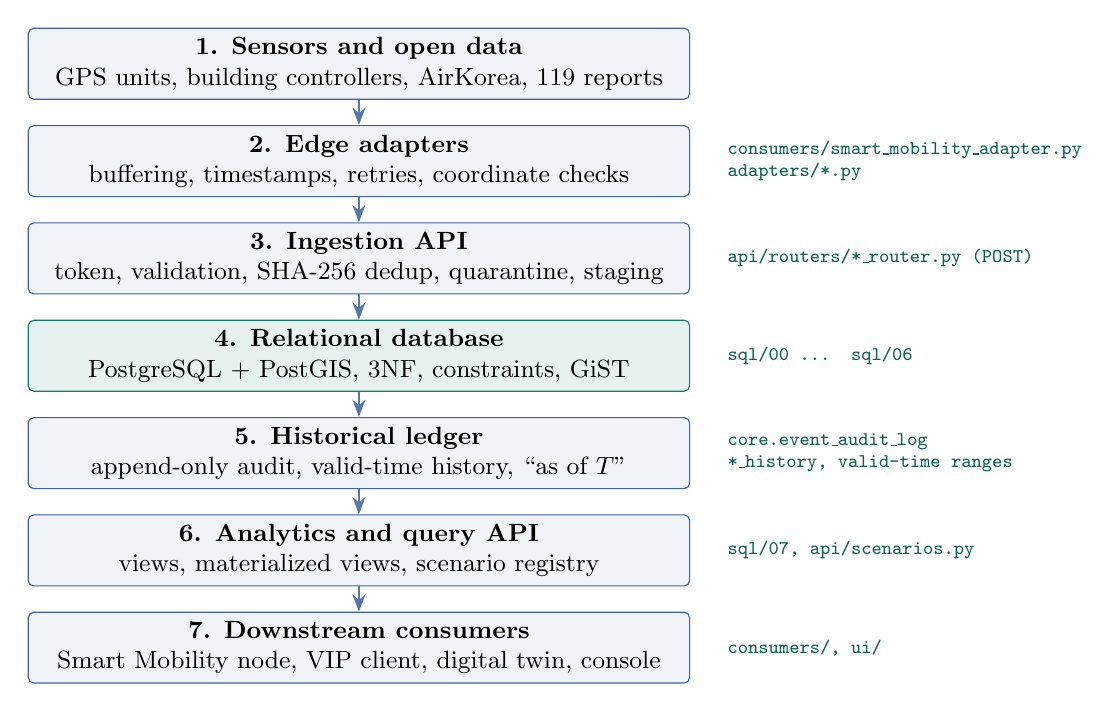
\begin{tikzpicture}[
  layer/.style={draw=inha!80,fill=inha!6,rounded corners=2pt,minimum width=8.4cm,
                minimum height=0.82cm,align=center,font=\small},
  side/.style={font=\scriptsize\ttfamily,align=left,text=accent!80!black,anchor=west},
  arr/.style={-{Stealth[length=2.2mm]},thick,inha!70},
  node distance=0.32cm]
\node[layer] (l1) {\textbf{1. Sensors and open data}\\ GPS units, building controllers, AirKorea, 119 reports};
\node[layer,below=of l1] (l2) {\textbf{2. Edge adapters}\\ buffering, timestamps, retries, coordinate checks};
\node[layer,below=of l2] (l3) {\textbf{3. Ingestion API}\\ token, validation, SHA-256 dedup, quarantine, staging};
\node[layer,below=of l3,fill=accent!10,draw=accent] (l4) {\textbf{4. Relational database}\\ PostgreSQL + PostGIS, 3NF, constraints, GiST};
\node[layer,below=of l4] (l5) {\textbf{5. Historical ledger}\\ append-only audit, valid-time history, ``as of $T$''};
\node[layer,below=of l5] (l6) {\textbf{6. Analytics and query API}\\ views, materialized views, scenario registry};
\node[layer,below=of l6] (l7) {\textbf{7. Downstream consumers}\\ Smart Mobility node, VIP client, digital twin, console};
\foreach \a/\b in {l1/l2,l2/l3,l3/l4,l4/l5,l5/l6,l6/l7} \draw[arr] (\a) -- (\b);
\node[side,right=0.35cm of l2] {consumers/smart\_mobility\_adapter.py\\adapters/*.py};
\node[side,right=0.35cm of l3] {api/routers/*\_router.py (POST)};
\node[side,right=0.35cm of l4] {sql/00 ... sql/06};
\node[side,right=0.35cm of l5] {core.event\_audit\_log\\{}*\_history, valid-time ranges};
\node[side,right=0.35cm of l6] {sql/07, api/scenarios.py};
\node[side,right=0.35cm of l7] {consumers/, ui/};
\end{tikzpicture}
\caption{The seven layers and where each one lives in the repository.}\label{fig:arch}
\end{figure}

\begin{table}[htbp]
\centering\small
\caption{Layer responsibilities and their implementation.}\label{tab:layers}
\begin{tabularx}{\linewidth}{@{}p{3.3cm}Xp{4.6cm}@{}}
\toprule
Layer & Responsibility & Implementation \\
\midrule
Edge adapters & Parse a source format, attach \code{observed_at}, buffer and retry & \code{adapters/*_adapter.py}, \code{consumers/smart_mobility_adapter.py} \\
Ingestion API & Authenticate, validate with Pydantic, run the pipeline, report the outcome & \cmd{POST /api/v1/...} in \code{api/routers/} \\
Relational database & Normalized schemas with keys, CHECK, FK, exclusion constraints, GiST indexes & \code{sql/00_init_database.sql} to \code{sql/06_db5_safety.sql} \\
Historical ledger & Append-only audit log, status history, valid-time intervals & \code{core.event_audit_log}, \code{safety.incident_status_history}, \code{building.device_space_assignments} \\
Analytics & Cross-domain views, materialized views with a logged refresh policy & \code{sql/07_cross_domain_views.sql} \\
Query API & Read endpoints and the scenario registry (bound parameters, read-only) & \code{api/scenarios.py}, \code{api/routers/} \\
Consumers & Programs that use only HTTP & \code{consumers/}, \code{ui/} \\
\bottomrule
\end{tabularx}
\end{table}

\subsection{Schemas}

Each domain has its own schema, so a team can work without touching the others, and
cross-domain joins are explicit:

\begin{center}\small
\begin{tabularx}{\linewidth}{@{}lX@{}}
\toprule
Schema & Content \\
\midrule
\code{core} & Source registry, canonical places, study area, ingestion batches, staging, quarantine, audit ledger \\
\code{mobility} & DB1: stops, routes and ordered patterns, vehicles, trips, stop events, GPS observations \\
\code{building} & DB2: buildings, space tree, devices, valid-time device locations, telemetry, maintenance \\
\code{tourism} & DB3: attractions, weekly opening hours, events, monthly totals, hourly samples \\
\code{environment} & DB4: stations, pollutant types, measurements, hourly rollup, alert rules and episodes \\
\code{safety} & DB5: facilities, incident types, severity levels, incidents, status history, drills \\
\code{cross_domain} & Three federated views, three materialized views and the refresh log \\
\bottomrule
\end{tabularx}
\end{center}

\subsection{Write path and read path}

The assignment asks for a separation between the two paths.

\begin{description}[leftmargin=0pt,style=nextline]
  \item[Write path.] A \code{POST} request is validated by Pydantic (types, ranges, time zone
    offset required). It then goes through an adapter, which runs the pipeline of
    Section~\ref{sec:pipeline} inside one database transaction, and returns
    \cmd{202 Accepted} with an outcome: \code{LOADED}, \code{DUPLICATE} or
    \code{QUARANTINED}.
  \item[Read path.] A \code{GET} endpoint or a scenario runs parameterized SQL in a
    \cmd{READ ONLY} transaction. Spatial filters use \code{ST_DWithin} on
    \code{geography} with a matching GiST expression index, and point-in-time questions bind
    $T$ as a parameter. The heaviest aggregates are served from materialized views.
\end{description}

% =============================================================================
\section{Technical baseline and repository}\label{sec:baseline}

\subsection{Versions}

\begin{table}[htbp]
\centering\small
\caption{Component versions: assignment baseline, development machine and hosted demo.}\label{tab:versions}
\begin{tabularx}{\linewidth}{@{}lXXX@{}}
\toprule
Component & Assignment baseline & Development (evidence run) & Hosted demo \\
\midrule
PostgreSQL & 16.3 & 18.3 (Windows 11) & 18.7 (Neon) \\
PostGIS & 3.4 & 3.7.0 & 3.6.4 \\
Python & 3.10+ & 3.14.4 & 3.12 (Docker image) \\
Driver & psycopg 3.3+ with pool & psycopg 3.3.9, psycopg-pool 3.3.3 & same \\
API & FastAPI 0.110+, Pydantic v2 & FastAPI 0.162.7, Pydantic 2.14.3, Uvicorn 0.54.0 & same \\
Web console & (not in baseline) & React 19.3, Vite 7.3, Leaflet 1.9.4 & built in the image \\
Reference system & WGS84 (EPSG:4326) & EPSG:4326, distances on \code{geography} & same \\
\bottomrule
\end{tabularx}
\end{table}

\subsection{Repository structure}

\begin{lstlisting}[basicstyle=\ttfamily\scriptsize]
Songdo-Urban-Digital-Memory/
  sql/00_init_database.sql ... 07_cross_domain_views.sql   migrations, run in order
  fixtures/seed_fixtures.py   deterministic generator (seed 20261002) -> seed_data.sql
  fixtures/songdo_stops.csv   513 real stops extracted from the MOLIT file
  adapters/                   base_adapter.py + one adapter per domain
  api/main.py, config.py, database.py, scenarios.py (36 tasks)
  api/routers/                core, mobility, building, tourism, environment, safety,
                              cross, scenario, system
  consumers/                  smart_mobility_adapter.py, vip_building_env_client.py,
                              digital_twin_temporal_replay.py, api_client.py
  ui/                         React + Vite + Leaflet console (served by FastAPI from ui/dist)
  scripts/                    setup_db.py, ingest_bus_stops.py, ingest_airkorea.py,
                              evidence.py, evidence_acceptance.py
  tests/test_platform.py      72 tests
  outputs/evidence/           generated evidence (reports, CSV, plans, screenshots)
  source_registry.csv         master data registry
  Dockerfile, render.yaml, compose.yaml, DEPLOY.md, README.md
  main.tex, main.pdf          this handbook
\end{lstlisting}

Secrets are kept out of the repository: \code{.env} (database password, AirKorea key, API
token) is git-ignored and \code{.env.example} holds placeholders only.

% =============================================================================
\section{Data sources and provenance}\label{sec:sources}

\subsection{Verification levels}

Every dataset that may enter the platform is registered in \code{core.source_registry}
(loaded from \code{source_registry.csv}), and every domain row carries the \code{source_id}
it came from. The registry gives each source a verification level and a provenance class:
\code{OFFICIAL_OPEN_DATA}, \code{CURATED_MANUAL} or \code{SYNTHETIC_FIXTURE}. A query can
therefore always tell real data from generated data.

\begingroup\small
\begin{xltabular}{\linewidth}{@{}p{2.3cm}Xcp{3.2cm}@{}}
\caption{Master source registry (15 sources).}\label{tab:sources}\\
\toprule
Source & Dataset & Level & Provenance \\
\midrule
\endfirsthead
\toprule
Source & Dataset & Level & Provenance \\
\midrule
\endhead
\code{SRC_CORE_01} & Curated Songdo landmark list (team) & 2 & CURATED\_MANUAL \\
\code{SRC_MOB_01} & Incheon bus stop information (Incheon City) & 4 & OFFICIAL\_OPEN\_DATA \\
\code{SRC_MOB_02} & Incheon bus route information (Incheon City) & 2 & OFFICIAL\_OPEN\_DATA \\
\code{SRC_MOB_03} & National bus stop locations (MOLIT, data.go.kr 15067528) & 4 & OFFICIAL\_OPEN\_DATA \\
\code{SRC_MOB_SYN} & Synthetic timetable and vehicle telemetry & 4 & SYNTHETIC\_FIXTURE \\
\code{SRC_BLD_01} & Building register (MOLIT / VWorld) & 2 & OFFICIAL\_OPEN\_DATA \\
\code{SRC_BLD_SYN} & Synthetic smart-building IoT data & 4 & SYNTHETIC\_FIXTURE \\
\code{SRC_TOU_01} & National tourist attraction standard data & 4 & OFFICIAL\_OPEN\_DATA \\
\code{SRC_TOU_02} & Incheon tourism visitor statistics & 3 & OFFICIAL\_OPEN\_DATA \\
\code{SRC_TOU_SYN} & Synthetic tourism data & 4 & SYNTHETIC\_FIXTURE \\
\code{SRC_ENV_01} & AirKorea air pollution information (KECO, 15073861) & 4 & OFFICIAL\_OPEN\_DATA \\
\code{SRC_ENV_02} & AirKorea monitoring stations (KECO, 15073877) & 4 & OFFICIAL\_OPEN\_DATA \\
\code{SRC_ENV_SYN} & Synthetic air-quality readings & 4 & SYNTHETIC\_FIXTURE \\
\code{SRC_SAF_01} & Incheon fire stations and 119 safety centers & 4 & OFFICIAL\_OPEN\_DATA \\
\code{SRC_SAF_02} & Synthetic incident response drill data & 4 & SYNTHETIC\_FIXTURE \\
\bottomrule
\end{xltabular}
\endgroup

\subsection{What is real and what is generated}

\begin{description}[leftmargin=0pt,style=nextline]
  \item[Real.] The 513 Songdo bus stops (IDs, names, coordinates) come from the national
    MOLIT stop file. \code{scripts/ingest_bus_stops.py} reads all 9,657 Incheon rows: it
    loads 513, quarantines 8,935 outside the Songdo box and 209 copies published by a second
    bus information system, and a second run changes nothing. The five AirKorea stations
    in the box are real, and \code{scripts/ingest_airkorea.py} ingests real hourly readings
    from the live API (or from an archived sample without a key).
  \item[Generated.] Routes, vehicles, trips and GPS tracks; building interiors and
    telemetry; opening hours, events and visitor counts; incidents and drills. They are
    produced by \code{fixtures/seed_fixtures.py} with the fixed seed \code{20261002}, so
    every run yields byte-identical \code{seed_data.sql}, and they are labelled with the
    \code{*_SYN} sources. The ``Route~8'' pattern is a corridor snapped to real stops, not
    the real Route~8.
  \item[Curated.] The 15 landmark coordinates were typed by hand and are approximate.
\end{description}

\subsection{Study area}

The Songdo teaching bounding box (longitude 126.600--126.685, latitude 37.350--37.425) is
stored once as a polygon in \code{core.study_areas}. It is exposed through
\code{core.songdo_bbox()} and \code{core.is_in_songdo(geom)}, and its values are also
configurable in \code{.env}. Every adapter checks coordinates against it. A latitude
around 126 or a longitude around 37 is reported as \code{COORDINATE_SWAPPED} rather than
as a generic out-of-bounds error.

\subsection{Seed data volume}

\begin{center}\small
\begin{tabular}{@{}lrlr@{}}
\toprule
Table & Rows & Table & Rows \\
\midrule
\code{mobility.stops} & 513 & \code{safety.incidents} & 10,006 \\
\code{mobility.trips} & 440 & \code{safety.incident_status_history} & 49,421 \\
\code{mobility.trip_stop_events} & 3,741 & \code{safety.response_drills} & 1,998 \\
\code{mobility.vehicle_observations} & 20,238 & \code{environment.measurements} & 8,640 \\
\code{building.telemetry} & 8,610 & \code{environment.hourly_summaries} & 720 \\
\code{tourism.sample_visits} & 6,696 & \textbf{All 39 tables} & \textbf{111,543} \\
\bottomrule
\end{tabular}
\end{center}

% =============================================================================
\section{Data model: entity-relationship diagrams}\label{sec:erd}

The diagrams in this section are generated by \cmd{python scripts/erd.py} from the PostgreSQL
catalog of the running database, not drawn by hand, so they always match the deployed schema.
The same diagrams, with a table of every key and constraint, are in \code{docs/erd/README.md},
which GitHub renders directly.

\subsection{Notation}

The domain diagrams use crow's-foot notation. Each box is a table, with its columns, types
and keys. \texttt{PK} marks the primary key, \texttt{FK} a foreign key, and \texttt{UK} a
single-column unique key. Comments mark \texttt{nullable} and \texttt{generated} columns.
Each line is a foreign key, labelled with the referencing column(s):

\begin{center}\small
\begin{tabularx}{\linewidth}{@{}p{3.6cm}X@{}}
\toprule
End of the line & Meaning \\
\midrule
Two bars at the parent & Mandatory: the foreign key is \texttt{NOT NULL}, every child has a parent \\
Bar and circle at the parent & Optional: the foreign key is nullable \\
Circle and crow's foot at the child & A parent has zero or more children (one-to-many) \\
Circle and bar at the child & A parent has at most one child (the foreign key is also unique: one-to-one) \\
\bottomrule
\end{tabularx}
\end{center}

A table from another schema is shown with its key only. Every domain table references
\code{core.source_registry} through \code{source_id}, which records the provenance of each row.

\subsection{Size of the model}

\begin{center}\small
\begin{tabular}{@{}lrrrrl@{}}
\toprule
Schema & Tables & FKs & Exclusion & Self-reference & Notes \\
\midrule
\code{core} & 7 & 7 & -- & -- & shared contracts and pipeline \\
\code{mobility} & 7 & 13 & 1 & -- & composite keys for stop order and stop events \\
\code{building} & 7 & 10 & 1 & 1 & space tree (room \ra{} floor) \\
\code{tourism} & 5 & 9 & 1 & -- & two visitor grains kept apart \\
\code{environment} & 6 & 10 & -- & -- & alert episodes reference their rule \\
\code{safety} & 6 & 9 & -- & -- & one-to-one drill \ra{} incident \\
\code{cross_domain} & 1 & -- & -- & -- & plus 4 views and 3 materialized views \\
\midrule
Total & 39 & 58 & 3 & 1 & \\
\bottomrule
\end{tabular}
\end{center}

\erdfigure[0.72\textheight]{overview}{Schema map: all 39 tables grouped by schema. Only links that cross a
schema boundary are drawn; a dashed line stands for the \texttt{source\_id} reference of every
table in that schema.}{fig:erd-overview}

\erdfigure{core}{ER diagram of the core schema: source registry, places, study area and the
ingestion pipeline (batches, staging, quarantine, audit ledger).}{fig:erd-core}

\erdfigure{mobility}{ER diagram of DB1 Mobility. \texttt{route\_stops} and
\texttt{trip\_stop\_events} have composite primary keys that give a gap-free order;
lateness and dwell are generated columns.}{fig:erd-mobility}

\erdfigure{building}{ER diagram of DB2 Smart Building. \texttt{spaces} references itself
(a room's parent floor, constrained to the same building); a device's location is the
valid-time table \texttt{device\_space\_assignments}, not a column of \texttt{devices}.}{fig:erd-building}

\erdfigure{tourism}{ER diagram of DB3 Tourism. Monthly totals (\texttt{aggregate\_visits}) and
hourly samples (\texttt{sample\_visits}) are separate tables because their grain differs.}{fig:erd-tourism}

\erdfigure{environment}{ER diagram of DB4 Environment. Hourly summaries and alert episodes are
derived from measurements; each alert references the rule it broke.}{fig:erd-environment}

\erdfigure{safety}{ER diagram of DB5 Safety and Incident. \texttt{incident\_status\_history} is the
append-only record of every status change; each drill belongs to exactly one incident
(one-to-one).}{fig:erd-safety}

\clearpage
% =============================================================================
\section{Core contracts and the ingestion pipeline}\label{sec:core}

\subsection{Core tables}

\begin{center}\small
\begin{tabularx}{\linewidth}{@{}p{4.4cm}X@{}}
\toprule
Table & Purpose \\
\midrule
\code{core.source_registry} & Every dataset with verification level, provenance and fallback strategy \\
\code{core.places} & Canonical places shared by all domains; \code{is_in_songdo} is a generated column computed from the geometry \\
\code{core.ingestion_batches} & One row per adapter run or API call, with received, loaded, duplicate and quarantined counts \\
\code{core.staging_records} & Raw payloads with their SHA-256 hash and status (\code{STAGED}, \code{LOADED}, \code{REJECTED}) \\
\code{core.quarantine_records} & Rejected payloads kept verbatim with a reason code and detail; never silently dropped \\
\code{core.event_audit_log} & Append-only ledger: one entry per loaded record with three timestamps \\
\bottomrule
\end{tabularx}
\end{center}

\subsection{The pipeline}\label{sec:pipeline}

All adapters inherit from \code{BaseAdapter} (\code{adapters/base_adapter.py}). A subclass
supplies only \code{validate()} and \code{load()}; the base class runs the same steps for
every domain:

\begin{enumerate}
  \item \textbf{Batch.} Open a row in \code{core.ingestion_batches}.
  \item \textbf{Hash.} Serialize the payload as canonical JSON (sorted keys, UTF-8 kept) and
    compute its SHA-256. The same record always gets the same hash, whatever its key order.
  \item \textbf{Deduplicate.} If this source already staged this hash for this table, count
    a duplicate and stop.
  \item \textbf{Validate.} Check the domain rules (bounding box, ranges, enumerations, time
    format). On failure, quarantine with a reason code.
  \item \textbf{Stage.} Insert the raw payload into \code{core.staging_records}.
  \item \textbf{Load and audit, atomically.} Inside a savepoint: insert or upsert the domain
    row, write the audit entry with \code{core.log_event()}, and mark the staging row
    \code{LOADED}. If any of the three fails, the savepoint rolls all three back. The staging
    row is then marked \code{REJECTED} and the payload quarantined with the database error
    (\code{FK_VIOLATION} or \code{SCHEMA_VIOLATION}). One bad record never aborts the batch.
\end{enumerate}

\begin{lstlisting}[language=Python,caption={The load step of \texttt{BaseAdapter.ingest()} (abridged).},captionpos=b]
try:
    with self.conn.transaction():  # savepoint: one bad row cannot abort the batch
        entity_id, action = self.load(cur, record)
        cur.execute("SELECT core.log_event(%s, %s, %s, %s, %s, %s, %s, %s, %s)",
                    (self.domain_schema, self.target_table, entity_id, action, observed_at,
                     received_at, self.source_id, Jsonb(record), self.actor))
        cur.execute("UPDATE core.staging_records SET status = 'LOADED', entity_id = %s "
                    "WHERE staging_id = %s", (entity_id, staging_id))
    summary.loaded += 1
except psycopg.Error as exc:
    cur.execute("UPDATE core.staging_records SET status = 'REJECTED' WHERE staging_id = %s",
                (staging_id,))
    reason = "FK_VIOLATION" if exc.sqlstate == "23503" else "SCHEMA_VIOLATION"
    self._quarantine(cur, summary, record, sha, received_at, reason, exc.diag.message_primary)
\end{lstlisting}

\subsection{Quarantine reason codes}

\begin{center}\small
\begin{tabularx}{\linewidth}{@{}p{4.3cm}X@{}}
\toprule
Reason code & Raised when \\
\midrule
\code{OUT_OF_BOUNDS} & The coordinate is outside the Songdo bounding box \\
\code{COORDINATE_SWAPPED} & Latitude and longitude are exchanged \\
\code{SCHEMA_VIOLATION} & A field is missing, malformed or outside its domain, or the database rejects the row \\
\code{FK_VIOLATION} & The record refers to an unknown entity (for example an unregistered vehicle) \\
\code{FAULT_READING} & AirKorea sends a fault marker (\code{-}) or a non-numeric value \\
\code{DUPLICATE_AUTHORITY} & A bus stop published by a second bus information system \\
\code{MISSING_FIELD}, \code{MISSING_COORDINATE}, \code{MALFORMED_COORDINATE} & A required value is absent or cannot be parsed \\
\bottomrule
\end{tabularx}
\end{center}

\subsection{Idempotency}

A record may arrive several times: a client retries after a timeout, or a source re-sends
its whole file. Three layers make re-delivery harmless:

\begin{enumerate}
  \item the staging check on \cmd{(source_id, target_table, payload_sha256)}, backed by
    \cmd{UNIQUE (batch_id, payload_sha256)}, reports a re-sent payload as \code{DUPLICATE};
  \item the domain tables have natural keys, such as \cmd{UNIQUE (vehicle_id, observed_at)}
    for GPS fixes and \cmd{UNIQUE (station_id, type_code, observed_at)} for measurements,
    and adapters write with \cmd{INSERT ... ON CONFLICT};
  \item quarantine rows are unique per \cmd{(source_id, payload_sha256, reason_code)}, so a
    repeatedly bad payload is stored once.
\end{enumerate}

The evidence run sent the same GPS packet four times (\code{LOADED}, then three times
\code{DUPLICATE}). It also sent 12 identical packets at the same moment from 12 threads.
In both cases exactly one row was stored.

\subsection{Append-only audit ledger}

\code{core.event_audit_log} keeps three timestamps per entry: \code{observed_at} (when the
event happened in the world), \code{received_at} (when the platform received it) and
\code{recorded_at} (when it was committed). Two triggers, \code{trg_audit_no_update_delete}
and \code{trg_audit_no_truncate}, call \code{core.forbid_mutation()}. It rejects
\code{UPDATE}, \code{DELETE} and \code{TRUNCATE} with SQLSTATE 23001, so history can only
grow. The same trigger protects \code{safety.incident_status_history}.

\begin{notebox}[Atomic write: evidence for the midterm P0 item]
The acceptance check CORE-2 replaces \code{core.log_event} inside the test transaction with
a function that always raises, then ingests a valid GPS packet. Result: 0 observation rows,
0 audit rows, the staging row is \code{REJECTED}, and the payload is quarantined with the
error. The batch still completes. A failure in the audit step therefore cannot leave a
domain row without its audit entry.
\end{notebox}

% =============================================================================
\section{DB1 Mobility}\label{sec:db1}

\subsection{Schema}

\begin{center}\small
\begin{tabularx}{\linewidth}{@{}p{4.5cm}X@{}}
\toprule
Table & Key design decisions \\
\midrule
\code{mobility.stops} & One row per physical stop pole; \code{stop_number} unique; point geometry with two GiST indexes (geometry and \code{geography} expression) \\
\code{mobility.routes}, \code{route_stops} & Ordered pattern: primary key \cmd{(route_id, direction, sequence_order)}; a stop appears once per direction \\
\code{mobility.vehicles} & Buses and autonomous shuttles, with capacity \\
\code{mobility.trips} & Exclusion constraint on \code{vehicle_id} and \cmd{tstzrange(departure, arrival)}: a vehicle cannot run two overlapping trips \\
\code{mobility.trip_stop_events} & Lateness and dwell are \cmd{GENERATED ALWAYS} columns, so they can never disagree with the timestamps \\
\code{mobility.vehicle_observations} & GPS history; \cmd{UNIQUE (vehicle_id, observed_at)}; GiST and B-tree indexes for space and time \\
\bottomrule
\end{tabularx}
\end{center}

\subsection{Scenarios}

\begin{center}\small
\begin{tabularx}{\linewidth}{@{}p{1.2cm}p{3.6cm}X@{}}
\toprule
ID & Question & Technique \\
\midrule
DB1-1 & Ordered stop sequence of a route & Composite primary key as a gap-free ordering; duplicate sequence rejected (23505) \\
DB1-2 & How did one trip run? & Generated columns for lateness and dwell; writing them directly is rejected (428C9) \\
DB1-3 & Where was every vehicle at $T$? & \cmd{DISTINCT ON (vehicle_id) ... ORDER BY vehicle_id, observed_at DESC} with $T$ bound \\
DB1-4 & Bunching and gaps in the peak & \code{LAG()} over \cmd{PARTITION BY route, direction, stop}; headway compared with schedule \\
DB1-5 & Which stops is a shuttle near? & Idempotent GPS ingestion, then \code{LATERAL} + \code{ST_DWithin} on \code{geography} \\
\bottomrule
\end{tabularx}
\end{center}

\subsection{Point-in-time replay (DB1-3)}

The platform never overwrites a vehicle's position; each GPS fix is a new row. The state at
any moment $T$ is reconstructed by keeping, per vehicle, the latest fix at or before $T$:

\begin{lstlisting}[language=PGSQL,caption={DB1-3: position of every vehicle as of $T$.},captionpos=b]
SELECT DISTINCT ON (o.vehicle_id)
       o.vehicle_id, v.vehicle_type, o.trip_id,
       ST_X(o.geom) AS lon, ST_Y(o.geom) AS lat, o.speed_kmh, o.observed_at,
       ROUND(EXTRACT(EPOCH FROM (%(as_of)s::timestamptz - o.observed_at)))::int AS staleness_seconds
FROM mobility.vehicle_observations o
JOIN mobility.vehicles v USING (vehicle_id)
WHERE o.observed_at <= %(as_of)s::timestamptz
ORDER BY o.vehicle_id, o.observed_at DESC
\end{lstlisting}

\cmd{DISTINCT ON} keeps the first row of each \code{vehicle_id} group in the
\cmd{ORDER BY} order. The second sort key, \cmd{observed_at DESC}, makes that first row
the latest fix. \cmd{UNIQUE (vehicle_id, observed_at)} rules out ties, so the answer is
deterministic. The acceptance check confirms that no returned fix is later than $T$, and
that a packet arriving afterwards leaves the answer for $T$ unchanged.

\subsection{Headway analysis (DB1-4)}

\begin{lstlisting}[language=PGSQL,caption={DB1-4: real headway between consecutive buses at each stop.},captionpos=b]
EXTRACT(EPOCH FROM e.observed_arrival - LAG(e.observed_arrival) OVER w)::int AS headway_seconds
...
WINDOW w AS (PARTITION BY t.route_id, t.direction, e.stop_id ORDER BY e.observed_arrival)
-- BUNCHED when headway < 0.75 x scheduled headway, GAP when > 1.25 x
\end{lstlisting}

In the morning peak (07:00--09:30) the task computes 181 headways across 19 trips. The
acceptance check recomputes the worst row independently and gets the same value (1,382 s).

\subsection{Telemetry ingestion and candidate stops (DB1-5)}

\cmd{POST /api/v1/mobility/observation} accepts one GPS fix. Pydantic rejects a speed
above 150 km/h, swapped coordinates, a malformed time and a time without a UTC offset,
all with 422. The adapter quarantines fixes outside Songdo and fixes from unknown
vehicles. For a vehicle's latest fixes, the task then finds the nearest stops within a
radius with \cmd{ST_DWithin(o.geom::geography, s.geom::geography, r)}.

\begin{notebox}[Boundary test]
Around the most isolated stop (the next one is 2,734 m away), a point 399 m away returns the
stop at a computed distance of 399.0 m, and a point 401 m away does not. The radius is
therefore applied in metres, not degrees.
\end{notebox}

% =============================================================================
\section{DB2 Smart Building}\label{sec:db2}

\subsection{Schema}

\begin{center}\small
\begin{tabularx}{\linewidth}{@{}p{4.9cm}X@{}}
\toprule
Table & Key design decisions \\
\midrule
\code{building.buildings} & Registry row linked to its canonical \code{core.places} row via \code{place_id} \\
\code{building.spaces} & Self-referencing tree (floor \ra{} room); a composite FK forces the parent to be in the same building \\
\code{building.devices} & Device master data; the location is \emph{not} stored here \\
\code{building.device_space_assignments} & Valid-time history: \cmd{[assigned_at, unassigned_at)} with an exclusion constraint \\
\code{building.telemetry} & Readings with a quality flag (\code{GOOD}/\code{SUSPECT}) against \code{metric_types} ranges \\
\code{building.maintenance_actions} & Work orders; an open action has \cmd{completed_at IS NULL} \\
\bottomrule
\end{tabularx}
\end{center}

\subsection{Scenarios}

\begin{center}\small
\begin{tabularx}{\linewidth}{@{}p{1.2cm}p{3.6cm}X@{}}
\toprule
ID & Question & Technique \\
\midrule
DB2-1 & Does each building match its canonical place? & Nearest place in metres; registry and place address shown side by side (\code{CONFIRMED}, \code{REVIEW}, \code{UNLINKED}) \\
DB2-2 & Floors, rooms and installed devices & Recursive space tree; orphan or cross-building parent rejected (23503) \\
DB2-3 & Where was a device at $T$? & Exclusion constraint on \code{tstzrange}; \code{building.relocate_device()} closes and opens intervals atomically \\
DB2-4 & Which devices went silent? & Last heartbeat per device before $T$; window $(T-15\,\mathrm{min},\,T]$; never-reported devices included \\
DB2-5 & VIP facility state & Latest reading per device with unit and age, open maintenance, current space \\
\bottomrule
\end{tabularx}
\end{center}

\subsection{Valid-time device location (DB2-3)}

A device moves between rooms over its life. Instead of a \code{space_id} column that is
overwritten, each stay is an interval:

\begin{lstlisting}[language=PGSQL,caption={No device can be in two places at once.},captionpos=b]
CREATE TABLE building.device_space_assignments (
    assignment_id  BIGSERIAL PRIMARY KEY,
    device_id      VARCHAR(48) NOT NULL REFERENCES building.devices(device_id),
    space_id       VARCHAR(48) NOT NULL REFERENCES building.spaces(space_id),
    assigned_at    TIMESTAMPTZ NOT NULL,
    unassigned_at  TIMESTAMPTZ,                     -- NULL = still installed
    CHECK (unassigned_at IS NULL OR unassigned_at > assigned_at),
    CONSTRAINT ex_assignment_no_overlap EXCLUDE USING GIST (
        device_id WITH =,
        tstzrange(assigned_at, unassigned_at) WITH &&
    )
);
\end{lstlisting}

\code{tstzrange} is half-open by default (\cmd{[start, end)}), so one stay may end exactly
when the next begins, but no two stays of a device may overlap. The constraint is enforced
by a GiST index (the \code{btree_gist} extension provides the \code{=} operator class).
Unlike a check done in application code, it also holds under concurrency.

\begin{notebox}[Race test (DB2-3-RACE)]
Two connections insert overlapping stays for the same device at the same time. The second
waits 0.50 s for the first to commit, then fails with \code{ExclusionViolation} (23P01).
Exactly one row is stored.
\end{notebox}

% =============================================================================
\section{DB3 Tourism}\label{sec:db3}

\subsection{Schema}

\begin{center}\small
\begin{tabularx}{\linewidth}{@{}p{4.4cm}X@{}}
\toprule
Table & Key design decisions \\
\midrule
\code{tourism.attractions} & Accessibility metadata (wheelchair, parking spaces, fee); linked to \code{core.places} \\
\code{tourism.operating_hours} & Several intervals per weekday allowed; overlapping intervals rejected by an exclusion constraint on \code{int4range} of minutes \\
\code{tourism.events} & Date range and daily times, CHECK that end $\ge$ start; cancelled events are kept with \code{is_cancelled} \\
\code{tourism.aggregate_visits} & Published monthly totals (grain: attraction $\times$ month) \\
\code{tourism.sample_visits} & Hourly sensor samples (grain: attraction $\times$ hour), deliberately a separate table \\
\bottomrule
\end{tabularx}
\end{center}

\subsection{Scenarios}

\begin{center}\small
\begin{tabularx}{\linewidth}{@{}p{1.2cm}p{3.6cm}X@{}}
\toprule
ID & Question & Technique \\
\midrule
DB3-1 & Accessible attractions & Filters on accessibility flags, nearest stop via \code{LATERAL}, source lineage \\
DB3-2 & Do events fit the venue's hours? & Range overlap against the weekday's opening intervals; \code{OUTSIDE_OPERATING_HOURS} flagged \\
DB3-3 & Official totals vs.\ samples & Two grains kept apart and compared side by side with coverage in percent \\
DB3-4 & What is open near a stop now? & Bound weekday, time and radius; \code{ST_DWithin} + opening interval containment \\
DB3-5 & Will transit cope with an event? & Expected attendance vs.\ seats of trips arriving within 500 m in the 2 hours before the start \\
\bottomrule
\end{tabularx}
\end{center}

\subsection{Why two visitor tables (DB3-3)}

Monthly totals and hourly samples have different grains and different sources. Storing
them in one table would invite adding hourly samples into a monthly total. The task shows
them side by side: the samples cover 28.7--39.9\,\% of the monthly totals. Every total is
labelled \code{SYNTHETIC_FIXTURE}, because no official tourism payload was archived (see
Section~\ref{sec:limits}).

\subsection{Open now, near transit (DB3-4)}

The acceptance check uses Convensia (open 09:00--18:00 on Fridays, 342 m from the stop). It
is returned at 17:59, not at 18:00 or 20:00, and not when the radius is 300 m. The closing
time is exclusive, and both the time and the distance limits are applied.

\subsection{Demand forecast (DB3-5)}

The task compares an event's expected attendance with the seats of all trips that arrive at
stops within 500 m in the 120 minutes before the event starts. Its stated assumption is
that every trip brings its full vehicle capacity. For example, EVT\_OUTLET\_SALE (5,000
visitors, 540 seats) is reported \code{OVER_CAPACITY}, and EVT\_BIO\_FORUM (800 visitors,
1,968 seats) \code{OK}.

% =============================================================================
\section{DB4 Environment}\label{sec:db4}

\subsection{Schema}

\begin{center}\small
\begin{tabularx}{\linewidth}{@{}p{4.6cm}X@{}}
\toprule
Table & Key design decisions \\
\midrule
\code{environment.stations} & The five real AirKorea stations inside the Songdo box \\
\code{environment.measurement_types} & Six criteria pollutants with unit and plausible range (outside = \code{SUSPECT}) \\
\code{environment.measurements} & \cmd{UNIQUE (station_id, type_code, observed_at)}; fault markers never reach this table \\
\code{environment.hourly_summaries} & Hourly average, minimum, maximum and count of \code{GOOD} values only \\
\code{environment.alert_rules} & Thresholds per pollutant and severity (\code{BAD}, \code{VERY_BAD}) \\
\code{environment.alerts} & Exceedance episodes: \code{ACTIVE} until an hour at or below the threshold follows \\
\bottomrule
\end{tabularx}
\end{center}

\subsection{Scenarios}

\begin{center}\small
\begin{tabularx}{\linewidth}{@{}p{1.2cm}p{3.6cm}X@{}}
\toprule
ID & Question & Technique \\
\midrule
DB4-1 & Stations, units and thresholds & Reference data with units; thresholds equal to the AirKorea grade boundaries \\
DB4-2 & Latest good reading per pollutant & \cmd{DISTINCT ON (type_code)} filtered on \cmd{quality_flag = 'GOOD'} \\
DB4-3 & Faults, late packets, corrections & Fault markers quarantined; late packets flagged by \code{received_at}; corrections upserted and audited as \code{UPDATE} \\
DB4-4 & Hourly rollup and alerts & \code{environment.refresh_hourly_summaries()} and \code{evaluate_alerts()} build and close episodes \\
DB4-5 & Air quality at any point & Nearest station by \code{geography} distance, latest readings with age and grade \\
\bottomrule
\end{tabularx}
\end{center}

\subsection{Real AirKorea data}

The station list of the AirKorea API has a trap: its field \code{dmX} holds the
\emph{latitude} and \code{dmY} the \emph{longitude}. The station adapter maps them
explicitly, and a test guards the mapping. One API row carries six pollutants, so the
reading adapter turns it into six measurements. AirKorea writes midnight as
\code{24:00} of the previous day, which the parser converts correctly. Readings sent as
\code{-} are quarantined as \code{FAULT_READING}.

\subsection{Alert thresholds (DB4-4)}

\begin{center}\small
\begin{tabular}{@{}lrrl@{}}
\toprule
Pollutant & BAD $>$ & VERY\_BAD $>$ & Unit \\
\midrule
PM10 & 80 & 150 & \(\mu\)g/m\textsuperscript{3} \\
PM2.5 & 35 & 75 & \(\mu\)g/m\textsuperscript{3} \\
O\textsubscript{3} & 0.090 & 0.150 & ppm \\
NO\textsubscript{2} & 0.060 & 0.200 & ppm \\
CO & 9 & 15 & ppm \\
SO\textsubscript{2} & 0.050 & 0.150 & ppm \\
\bottomrule
\end{tabular}
\end{center}

The acceptance check feeds an hourly PM2.5 average of exactly 75 (only \code{BAD} is
raised, because \code{VERY_BAD} needs a value above 75), then 76 (both raised), then clean
hours, which resolve the episodes.

% =============================================================================
\section{DB5 Safety and Incident}\label{sec:db5}

\subsection{Schema}

\begin{center}\small
\begin{tabularx}{\linewidth}{@{}p{4.9cm}X@{}}
\toprule
Table & Key design decisions \\
\midrule
\code{safety.facilities} & Fire stations, 119 safety centers and police boxes \\
\code{safety.incident_types}, \code{severity_levels} & Responder per type, default restriction radius; SLA target per severity (CRITICAL 300 s \dots{} LOW 900 s) \\
\code{safety.incidents} & Current state; \code{current_status} changes only through \code{safety.transition_incident()} \\
\code{safety.incident_status_history} & Append-only log of every change; the status at any past $T$ is read from here \\
\code{safety.response_drills} & Exercises scored by the database against a target time \\
\bottomrule
\end{tabularx}
\end{center}

\subsection{Scenarios}

\begin{center}\small
\begin{tabularx}{\linewidth}{@{}p{1.3cm}p{3.5cm}X@{}}
\toprule
ID & Question & Technique \\
\midrule
DB5-1 & Facilities and their workload & Reference data with nearest stop and incident counts \\
DB5-2 & Triage of new incidents & Validated report (severity enumeration), ordered by severity rank and SLA \\
DB5-3 & Lifecycle of an incident & State machine in SQL: transition function with row lock, guard trigger, history trigger \\
DB5-4 & Response time by facility & Durations from the history (report \ra{} on scene), average and percentiles, SLA met \\
DB5-4B & Incident hotspots & \code{ST_ClusterDBSCAN} in a metric projection (EPSG:5186), deterministic membership \\
DB5-5 & Hazard zones for path planners & Incidents active at $T$, buffer on \code{geography}, GeoJSON polygon, stops and vehicles inside \\
\bottomrule
\end{tabularx}
\end{center}

\subsection{State machine (DB5-3)}

\begin{center}
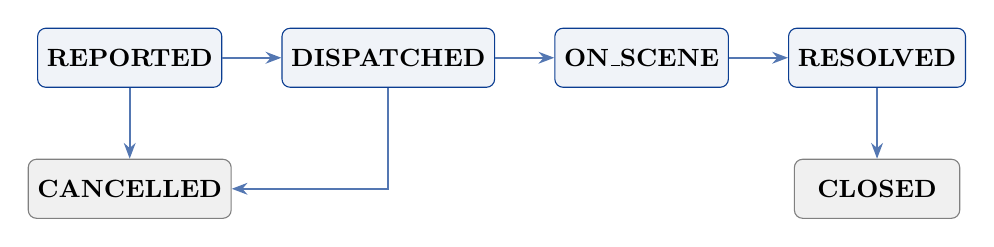
\begin{tikzpicture}[
  st/.style={draw=inha,fill=inha!6,rounded corners=3pt,minimum height=0.75cm,minimum width=2.1cm,font=\small\bfseries},
  fin/.style={st,fill=gray!12,draw=gray},
  arr/.style={-{Stealth[length=2mm]},thick,inha!70},
  node distance=0.75cm]
\node[st] (rep) {REPORTED};
\node[st,right=of rep] (dis) {DISPATCHED};
\node[st,right=of dis] (ons) {ON\_SCENE};
\node[st,right=of ons] (res) {RESOLVED};
\node[fin,below=0.9cm of res] (clo) {CLOSED};
\node[fin,below=0.9cm of rep] (can) {CANCELLED};
\draw[arr] (rep) -- (dis); \draw[arr] (dis) -- (ons); \draw[arr] (ons) -- (res); \draw[arr] (res) -- (clo);
\draw[arr] (rep) -- (can); \draw[arr] (dis) |- (can);
\end{tikzpicture}
\end{center}

The allowed steps are defined once, in \cmd{safety.valid_incident_transition(from, to)}.
Three objects enforce them:

\begin{itemize}
  \item \code{safety.transition_incident()} locks the incident row with
    \cmd{SELECT ... FOR UPDATE} and checks the step. A dispatch also requires a facility,
    and a change may not be dated before the previous one. Only then does it update the
    status.
  \item The trigger \code{trg_incidents_status_guard} rejects any \code{UPDATE} that
    bypasses the function with an illegal step (SQLSTATE 23514).
  \item The trigger \code{trg_incidents_status_log} writes the history row in the same
    statement, so the status and its history cannot diverge.
\end{itemize}

\begin{lstlisting}[language=PGSQL,caption={Core of \texttt{safety.transition\_incident()} (abridged).},captionpos=b]
SELECT current_status, assigned_facility_id INTO v_current, v_assigned
FROM safety.incidents WHERE incident_id = p_incident_id
FOR UPDATE;                                   -- concurrent transitions queue here
IF NOT FOUND THEN
    RAISE EXCEPTION 'unknown incident %', p_incident_id USING ERRCODE = 'no_data_found';
END IF;
IF NOT safety.valid_incident_transition(v_current, p_to_status) THEN
    RAISE EXCEPTION 'incident %: transition % -> % is not allowed',
          p_incident_id, v_current, p_to_status USING ERRCODE = 'check_violation';
END IF;
...
UPDATE safety.incidents
SET current_status = p_to_status,
    assigned_facility_id = COALESCE(p_facility_id, assigned_facility_id)
WHERE incident_id = p_incident_id;           -- the history trigger appends the change
\end{lstlisting}

The API maps a rejected step to \cmd{409 Conflict}. The acceptance results:
\code{REPORTED \ra{} RESOLVED} is rejected; a plain \code{UPDATE} that skips states is
rejected by the trigger; deleting history is rejected (23001); an accepted dispatch writes
the status and one history row together.

\begin{notebox}[Race test (DB5-3-RACE)]
Two connections dispatch the same \code{REPORTED} incident at the same moment. The second
waits 0.51 s on the row lock. It then sees \code{DISPATCHED}, for which a second
\code{DISPATCHED} is not a legal step, and fails with 23514. The history holds exactly
one \code{DISPATCHED} row.
\end{notebox}

\subsection{Status at any past moment}

Because every change is in the history, ``which incidents were active at 18:20?'' is
answered without guessing. For each incident, the query takes the last history row with
\cmd{changed_at <= T} (ordered by \cmd{changed_at DESC, history_id DESC} for a total
order) and keeps those whose status was \code{REPORTED}, \code{DISPATCHED} or
\code{ON_SCENE}. The same rule drives the console's time slider.

\subsection{Hazard zones (DB5-5)}

For every incident active at $T$ with a restriction radius, the task returns the zone as a
GeoJSON polygon (\code{ST_Buffer} on \code{geography}, so the radius is in metres), with
the stops and moving vehicles inside it. In the acceptance check, a fire with a 300 m
restriction produces a closed 33-point polygon. After the incident is \code{RESOLVED} at
19:00, the zone is gone at 19:30, but still appears when 18:30 is replayed.

\subsection{Hotspots (DB5-4B)}

DBSCAN clustering needs a distance in metres, so the points are transformed to the Korean
metric projection EPSG:5186 before \code{ST_ClusterDBSCAN}. Two runs give identical
membership (5 clusters, largest 1,440 incidents).

% =============================================================================
\section{Cross-domain federation}\label{sec:cross}

\code{sql/07_cross_domain_views.sql} joins the domains through space and time. It does not
copy data between schemas.

\begin{center}\small
\begin{tabularx}{\linewidth}{@{}p{6.4cm}X@{}}
\toprule
Object & Question it answers \\
\midrule
\code{v_attractions_events_near_stops} & Which attractions and events are within 500 m of each stop? (mobility $\times$ tourism) \\
\code{v_building_devices_with_environmental_context} & What is the outdoor PM at the station nearest to each building? (building $\times$ environment) \\
\code{v_incidents_mobility_environmental_impact} & Which stops are within 600 m of an open incident, and is there an air alert nearby? (safety $\times$ mobility $\times$ environment) \\
\code{mv_place_context} (materialized) & One context card per place: nearest stop, station, fire and police unit, counts within 500 m \\
\code{mv_facility_response_stats} (materialized) & Monthly response statistics per facility (average, median, p90, SLA met) \\
\code{mv_stop_hourly_service} (materialized) & Arrivals, seats, lateness and boardings per stop and hour \\
\bottomrule
\end{tabularx}
\end{center}

Figure~\ref{fig:erd-lineage} shows which tables each view reads.

\erdfigure[0.78\textheight]{cross_domain}{Lineage of the cross-domain views (rounded) and
materialized views (double border): the tables each one reads, by schema.}{fig:erd-lineage}

\subsection{Refresh policy}

\code{cross_domain.refresh_materialized_views()} refreshes each view with
\cmd{REFRESH MATERIALIZED VIEW CONCURRENTLY}. Each view has a unique index, so readers
are never blocked. Every refresh is logged in \code{cross_domain.refresh_log} with its
duration and row count, and \code{v_materialized_view_freshness} reports how old each view
is. The API exposes \cmd{POST /api/v1/cross/refresh} and \cmd{GET .../freshness}. The
acceptance check X-MV refreshes, then compares the facility statistics view with the live
aggregate for all five facilities. They are equal.

\subsection{``Nearest'' means nearest in metres}

Ten queries first ranked ``nearest'' with the KNN operator \cmd{geom <-> geom} on
EPSG:4326 geometries. That operator measures in degrees. At Songdo's latitude
(37.4$^\circ$N) one degree of longitude is only about 0.79 of a degree of latitude in
length, so the ranking is distorted. For one landmark it picked a station 1,722 m away
instead of one 1,478 m away. The evidence run found this, and all ten queries now order by
\cmd{ST_Distance(a.geom::geography, b.geom::geography)}. The check X-VIEWS confirms that
every device's station is the true nearest one.

% =============================================================================
\section{Data services: the REST API}\label{sec:api}

\subsection{Conventions}

\begin{itemize}
  \item Interactive documentation at \code{/docs} (OpenAPI, 53 paths).
  \item Write endpoints require the header \code{X-API-Token}; without it they return 401.
  \item Ingestion endpoints return \cmd{202 Accepted} with \code{LOADED},
    \code{DUPLICATE} or \code{QUARANTINED} and the batch counters. Malformed requests get
    422, an illegal state change 409, an unknown task 404.
  \item All SQL is parameterized (psycopg binds values); no request value is ever
    formatted into SQL text.
  \item Scenario SQL runs in a \cmd{READ ONLY} transaction.
  \item \cmd{GET /health} returns 503 when the database is unreachable, which is also
    what the hosted deployment uses as its health check.
\end{itemize}

\subsection{Endpoints}

\begingroup\small
\begin{xltabular}{\linewidth}{@{}p{1.5cm}Xp{1.6cm}@{}}
\caption{Main endpoints (all under \texttt{/api/v1}).}\label{tab:endpoints}\\
\toprule
Method & Path and purpose & Scenario \\
\midrule
\endfirsthead
\toprule
Method & Path and purpose & Scenario \\
\midrule
\endhead
GET & \code{/core/places/nearby}: places within a radius in metres & CORE-1 \\
GET & \code{/core/sources}, \code{/core/quarantine}: registry and quarantine & CORE-2/3 \\
POST & \code{/core/places}: ingest places through the pipeline & CORE \\
GET & \code{/mobility/stops/nearby}, \code{/mobility/stops.geojson}: stops (GeoJSON export) & DB1 \\
GET & \code{/mobility/routes/<route>/stops}: ordered pattern & DB1-1 \\
GET & \code{/mobility/trips/<trip_id>/events}: arrivals with lateness and dwell & DB1-2 \\
GET & \code{/mobility/vehicles/positions?as_of=T}: positions at $T$ & DB1-3 \\
POST & \code{/mobility/observation}: ingest one GPS fix & DB1-5 \\
GET & \code{/building/buildings/<id>/state}: facility state for VIP & DB2-5 \\
GET & \code{/building/devices/silent}, \code{/building/devices/<id>/history} & DB2-4/3 \\
POST & \code{/building/devices/<id>/relocate}, \code{/building/telemetry} & DB2 \\
GET/POST & \code{/tourism/attractions}, \code{/tourism/attractions/open}, \code{/tourism/events} & DB3-1/4/2 \\
GET & \code{/tourism/attractions/<id>/visits}: totals vs.\ samples & DB3-3 \\
GET & \code{/environment/stations}, \code{.../<name>/latest}, \code{.../measurements} & DB4-1/2 \\
GET & \code{/environment/exposure}, \code{/environment/alerts} & DB4-5/4 \\
POST & \code{/environment/measurements}: ingest, then refresh rollup and alerts & DB4-3 \\
GET & \code{/safety/facilities}, \code{/safety/incidents/active?as_of=T}, \code{/safety/incidents/<id>} & DB5-1/3 \\
GET & \code{/safety/hazard-zones}, \code{/safety/analytics/response-times} & DB5-5/4 \\
POST & \code{/safety/incidents}, \code{/safety/incidents/<id>/transition} & DB5-2/3 \\
GET & \code{/cross/attractions-near-stops}, \code{/cross/building-context/<id>}, \code{/cross/incident-impact} & X-1/2/3 \\
GET & \code{/cross/place-context}, \code{/cross/facility-response-stats}, \code{/cross/freshness} & X-4/5/6 \\
POST & \code{/cross/refresh}: refresh materialized views & X \\
PATCH & \code{/core/places/<id>}, \code{/tourism/attractions/<id>}, \code{/tourism/events/<id>}, \code{/building/devices/<id>}: correct fields & edits \\
DELETE & same paths: delete if unreferenced (places, attractions), cancel (events), retire (devices) & edits \\
GET/POST & \code{/scenarios}, \code{/scenarios/<id>/run}: list and run any task & all \\
GET/POST & \code{/system/map/layers}, \code{/system/map/frame}, \code{/system/activity}, \code{/system/verification}, \code{/system/run-tests} & console \\
\bottomrule
\end{xltabular}
\endgroup

\subsection{Corrections and retirement}\label{sec:edits}

Reference data can be corrected (\code{PATCH}) and removed (\code{DELETE}). The platform is an
urban memory, so what ``delete'' means depends on the kind of data:

\begin{center}\small
\begin{tabularx}{\linewidth}{@{}p{3.6cm}XX@{}}
\toprule
Kind of data & PATCH & DELETE \\
\midrule
Places, attractions & Changed fields are written & Removed only when nothing refers to the row, otherwise 409; the audit entry keeps the full deleted row \\
Events & Changed fields are written & Soft delete: \code{is_cancelled = true}, the row stays \\
Devices & Fields and status (\code{ACTIVE}, \code{FAULT}, \code{MAINTENANCE}); a retired device is not edited (409) & Retire: status \code{RETIRED} and the open location interval closed now, so where the device was in the past is unchanged \\
History (GPS, telemetry, measurements) & Never edited in place; a corrected reading is re-sent through ingestion and replaces the value (DB4-3) & Not allowed \\
Audit ledger, status history & Blocked by trigger & Blocked by trigger \\
\bottomrule
\end{tabularx}
\end{center}

Every change runs in one transaction (\code{api/edits.py}): the row is locked with
\cmd{SELECT ... FOR UPDATE}, compared with the request, written, and recorded with
\code{core.log_event()}, whose entry holds the old and new values. A \code{PATCH} that changes
nothing returns \code{UNCHANGED} and writes nothing. If the audit write fails, the change is rolled
back as well. Coordinates are checked against the Songdo box (422), and the database's own
constraints still apply: for example, parking spaces without parking or an event ending before
it starts is rejected with 409.

\subsection{Scenario registry}

\code{api/scenarios.py} holds all 36 tasks in one dictionary. Each task has an ID, a title,
a summary, its SQL and typed parameters with defaults. Each parameter converts and checks
its value, so a bad date returns 422, not 500. The endpoint
\cmd{POST /api/v1/scenarios/<id>/run} runs a task and returns the rows, the SQL that ran
and its plan. Adding a scenario to the registry makes it appear in \code{/docs} and in the
console without further work.

% =============================================================================
\section{Downstream consumers}\label{sec:consumers}

The three consumers in \code{consumers/} use only HTTP, never the database. Each one talks
to the server at \code{SONGDO_API_URL}; if none is running, it starts the API inside its own
process.

\begin{description}[leftmargin=0pt,style=nextline]
  \item[Smart Mobility node (\code{smart_mobility_adapter.py}).] A ROS-style telemetry node.
    A driver thread moves a shuttle along a real route and publishes GPS fixes into a
    \emph{bounded} queue that drops the oldest fix when full, so the control loop never
    blocks. A separate uplink thread drains the queue to
    \cmd{POST /mobility/observation}. It retries network errors and 5xx responses with
    exponential backoff and never retries a 4xx. To exercise the pipeline, it injects a
    GPS glitch every 25th packet and re-sends every 40th.
  \item[VIP building client (\code{vip_building_env_client.py}).] Combines a building's
    indoor state (\code{/building/.../state}) with the outdoor air at that location
    (\code{/environment/exposure}). It gives a ventilation advice (a demonstration rule)
    with caveats, such as a device that has been silent for more than 30 minutes.
  \item[Digital twin replay (\code{digital_twin_temporal_replay.py}).] Rebuilds the city at
    any moment $T$: vehicle positions and incident statuses, every 5 minutes over a chosen
    interval, entirely from history.
\end{description}

% =============================================================================
\section{Integrated web console}\label{sec:ui}

The console (\code{ui/}, React + Vite + Leaflet) implements the professor's requirement of
a fully integrated interface for choosing and running any task. In production it is built
into \code{ui/dist} and served by FastAPI at \code{/}, so one process serves both the API
and the console.

\begin{center}\small
\begin{tabularx}{\linewidth}{@{}p{2.2cm}X@{}}
\toprule
Page & Function \\
\midrule
Tasks & All 36 tasks, searchable. Pick one, edit its parameters, run it: rows, the SQL that ran, the query plan, and a map when the result has coordinates. \\
City map & Stops, routes, stations, attractions, buildings and facilities. A time slider rebuilds the city at any moment from history: vehicles, incidents in their status at that time, PM2.5 grade per station, active air alerts. Live mode refreshes every 2 s. \\
Ingest & Eight forms, one per data-entry endpoint: a new place, a GPS fix, a building reading, a device relocation, a new attraction, an air reading, an incident report and a status change, each with valid and invalid presets. A ninth tab, \emph{Edit / retire}, corrects or deletes places, attractions, events and devices (Section~\ref{sec:edits}). Shows the outcome and the batch, quarantine and audit rows written. \\
Verify & 28 live platform checks (schemas, rows, views, freshness, ledger triggers, indexes, constraints) and a button that runs the test suite. \\
\bottomrule
\end{tabularx}
\end{center}

Pages can be opened in a given state by link, for example \code{#/tasks?task=DB5-2&run=1&view=map}
or \code{#/map?t=18:20}.

\evidencefigure{page_map_1820.png}{City map replayed at 18:20 on the fixture day: vehicles, incidents in their status at that moment, PM2.5 grade per station.}{fig:map}

\evidencefigure{page_task_result_map.png}{Tasks page: a task's result rows shown on the map.}{fig:taskmap}

\evidencefigure[0.85\linewidth]{page_ingest.png}{Ingest page: an invalid GPS fix is quarantined with its reason code.}{fig:ingest}

\evidencefigure[0.85\linewidth]{page_verify.png}{Verify page: live platform checks.}{fig:verify}

% =============================================================================
\section{Testing and verification}\label{sec:evidence}

\subsection{Automated test suite}

\cmd{python -m unittest tests/test_platform.py} runs 72 tests in about 5 seconds. Every
database test runs inside a transaction that is rolled back, so the suite leaves no trace
and can run against any copy of the database.

\begin{center}\small
\begin{tabularx}{\linewidth}{@{}p{4.6cm}rX@{}}
\toprule
Test class & Tests & What it covers \\
\midrule
CoordinateValidationTests & 4 & Valid point, out of bounds, swapped, malformed \\
PayloadHashTests, AirKoreaParsingTests & 3 & Key-order-independent hash, UTF-8, 24:00, six readings per row \\
ScenarioRegistryTests & 2 & All 25 scenarios registered, every ready one has SQL \\
ApiValidationTests & 23 & 422/401/404 handling (including edits), every scenario runs with defaults, each domain's endpoints, console and consumer endpoints \\
DatabaseTests & 4 & Bounding box function, pipeline, append-only ledger, GiST index use \\
Mobility- \dots{} SafetyDatabaseTests & 21 & Domain constraints, adapters, state machine, alerts, drills \\
CrossDomainDatabaseTests & 4 & Materialized view equals live query, logged refresh, index use \\
EditDatabaseTests & 6 & PATCH writes and audits only real changes; delete only when unreferenced; cancel and retire keep history; a failed audit rolls the change back \\
ConsumerTests & 5 & Bounded queue, route driver, fault injection, time parsing, retry policy \\
\bottomrule
\end{tabularx}
\end{center}

\subsection{The evidence kit}

\cmd{python scripts/evidence.py} (about 3.5 minutes) proves the platform end to end
without touching the developer's database:

\begin{enumerate}
  \item creates a new database \code{songdo_evidence} and runs every migration and the seed
    with \cmd{psql -v ON_ERROR_STOP=1};
  \item records the version of every component and the git commit;
  \item dumps it with \cmd{pg_dump -Fc}, restores into a second new database, and
    compares the two;
  \item runs the test suite and the acceptance checks against the new database;
  \item measures every task with \cmd{EXPLAIN (ANALYZE, BUFFERS)}, with and without index
    scans, and on a 1,000,000-row benchmark table;
  \item starts a real Uvicorn server and runs 24 API contract cases and a latency test;
  \item opens every task in headless Chrome and compares the rendered row count with the API;
  \item writes \code{outputs/evidence/README.md} and the CSV files, then drops both
    databases.
\end{enumerate}

\subsection{Acceptance matrix}

Each scenario has one executed check, written against the ``Required acceptance'' column
of the midterm feedback. Checks run in a rolled-back transaction, except the two races,
which commit on the disposable database. \limited{} means the check ran and passed, but
part of the criterion needs data the project does not have.

\begingroup\small
\begin{xltabular}{\linewidth}{@{}p{2.1cm}Xp{1.45cm}@{}}
\caption{Scenario acceptance results (29 PASS, 3 LIMITED, 0 FAIL).}\label{tab:acceptance}\\
\toprule
ID & Criterion and result & Status \\
\midrule
\endfirsthead
\toprule
ID & Criterion and result & Status \\
\midrule
\endhead
\bottomrule
\endfoot
CORE-1 & Re-delivery leaves one record; 4 records \ra{} 1 loaded, 2 quarantined (out of bounds, swapped), 1 duplicate; re-sent batch \ra{} 4 duplicates & \pass \\
CORE-2 & Failure in the audit step leaves no partial rows & \pass \\
CORE-3 & Ledger rejects UPDATE, DELETE, TRUNCATE (23001); three timestamps present & \pass \\
DB1-1 & 6 patterns ordered 1..n without gaps; duplicate sequence and repeated stop rejected & \pass \\
DB1-2 & Known event at +120 s / 30 s dwell computed by the database; direct write rejected & \pass \\
DB1-3 & $T$ bound; no fix after $T$; later packet does not change the answer & \pass \\
DB1-4 & 181 headways over 19 trips; worst row recomputed independently (1,382 s) & \pass \\
DB1-5 & Packet sent 3 times \ra{} 1 row; 399 m returned, 401 m not & \pass \\
DB2-1 & Linked place = nearest canonical place for all 5 buildings; test-bed reported UNLINKED & \pass \\
DB2-2 & Orphan and cross-building parent rejected; 13 installed devices = 13 open assignments & \pass \\
DB2-3 & Overlap rejected (23P01); adjacent intervals accepted; inverted interval rejected & \pass \\
DB2-3-RACE & Concurrent overlapping inserts: one waits, then fails; 1 row stored & \pass \\
DB2-4 & Never reported; exactly 15:00 old \ra{} silent; 14:59 old \ra{} not silent & \pass \\
DB2-5 & 13 devices with reading, unit, age, maintenance; relocated device in its new room & \pass \\
DB3-1 & 9 venues with accessibility flags and nearest stop; lineage reported & \pass \\
DB3-2 & Inverted dates rejected; event inside hours OK, 1 minute after closing flagged & \pass \\
DB3-3 & Totals and samples kept apart and compared; no archived official payload & \limited \\
DB3-4 & Convensia at 17:59 yes, 18:00 and 20:00 no, 300 m no & \pass \\
DB3-5 & Demand vs.\ seats with the assumption stated; 4 events classified & \pass \\
DB4-1 & Six units; thresholds cited by name, source document not archived & \limited \\
DB4-2 & Six pollutants loaded as GOOD; \code{-}, \code{abc}, empty quarantined & \pass \\
DB4-3 & Replay: load, duplicate, correction (logged as UPDATE), fault quarantined & \pass \\
DB4-4 & PM2.5 at 75 \ra{} BAD only; 76 \ra{} BAD + VERY\_BAD; clean hours resolve & \pass \\
DB4-5 & Nearest station checked by full scan (745.5 m); 6 readings with age & \pass \\
DB5-1 & 5 facilities inside the box; coordinates are placeholders & \limited \\
DB5-2 & Valid report \ra{} REPORTED with history; invalid severity quarantined / 422 & \pass \\
DB5-3 & Illegal step and bypassing UPDATE rejected; history delete rejected; atomic history & \pass \\
DB5-3-RACE & Concurrent dispatches: one waits on the row lock, then fails; one history row & \pass \\
DB5-4 & Average response recomputed independently (260 s); DBSCAN identical on two runs & \pass \\
DB5-5 & Zone published as closed polygon; gone after resolution, present when replayed & \pass \\
X-VIEWS & Distance caps (498.1 m $\le$ 500, 599.9 m $\le$ 600); true nearest station & \pass \\
X-MV & Materialized view equals live aggregate after a logged refresh & \pass \\
\end{xltabular}
\endgroup

\subsection{API contract}

\begin{center}\small
\begin{tabularx}{\linewidth}{@{}Xp{4.2cm}p{4.2cm}@{}}
\toprule
Case & Expected & Actual \\
\midrule
Valid GPS fix, then 3 retries & 202 LOADED, then DUPLICATE $\times$3 & as expected, 1 row \\
No token / wrong token & 401 & 401 \\
Speed 400 km/h; swapped coordinates; time without offset; malformed time; missing field & 422 & 422, 0 rows \\
Fix outside Songdo / unknown vehicle & 202 QUARANTINED & OUT\_OF\_BOUNDS / FK\_VIOLATION \\
Invalid severity & 422 & 422 \\
REPORTED \ra{} RESOLVED; CLOSED \ra{} DISPATCHED & 409 & 409 \\
REPORTED \ra{} DISPATCHED & 200 & 200, 2 history rows \\
Unknown task; bad parameter; negative radius & 404; 422; 422 & as expected \\
12 identical packets at once & 1 stored row & 1 LOADED, 11 DUPLICATE \\
PATCH a place, then the same value again & 200 UPDATED, then UNCHANGED & 1 audit entry \\
PATCH outside Songdo; unknown field; unknown place & 422; 422; 404 & as expected \\
DELETE a place in use; an unreferenced place & 409; 200 DELETED & row kept; row gone, full row in audit \\
DELETE an event; a device & 200 CANCELLED; 200 RETIRED & row kept; location closed, history kept \\
PATCH a retired device; parking without parking & 409; 409 & as expected \\
\bottomrule
\end{tabularx}
\end{center}

\subsection{Web console}

Each of the 36 tasks was opened in headless Chrome through its link. The row count read
from the rendered page matched the API for all 36.

% =============================================================================
\section{Performance}\label{sec:perf}

\subsection{Index versus no index at scale}

A benchmark copy of the GPS table with the same columns and indexes was filled with
1,000,000 rows (500 vehicles $\times$ 2,000 fixes, fixed random seed). Each query was timed
with the indexes (median of 5 runs) and with index scans disabled (median of 3 runs).

\begin{center}\small
\begin{tabularx}{\linewidth}{@{}Xrrr@{}}
\toprule
Query (1,000,000 rows) & With index (ms) & Without (ms) & Speed-up \\
\midrule
Radius search: fixes within 150 m of a point (GiST on \code{geography}) & 29.42 & 733.1 & 25$\times$ \\
Point-in-time replay: last fix of 50 vehicles at $T$ (B-tree \cmd{(vehicle_id, observed_at)}) & 1.30 & 3,847.7 & 2,961$\times$ \\
Time window: fixes in a 5-minute interval (B-tree \code{observed_at}) & 1.22 & 58.1 & 48$\times$ \\
\bottomrule
\end{tabularx}
\end{center}

\subsection{Index versus no index on the project data}

\begin{center}\small
\begin{tabularx}{\linewidth}{@{}Xrrr@{}}
\toprule
Query & Planner (ms) & No index (ms) & Speed-up \\
\midrule
Stops within 1,000 m (513 stops, \code{idx_stops_geog}) & 0.42 & 1.22 & 2.9$\times$ \\
GPS points within 150 m (20,238 rows, \code{idx_obs_geog}) & 4.61 & 36.20 & 7.9$\times$ \\
Last position of each vehicle at $T$ & 0.99 & 46.77 & 47.2$\times$ \\
Status history of one incident (49,421 rows) & 0.18 & 4.97 & 27.4$\times$ \\
Audit history of one entity (small table: the index costs more than it saves) & 0.29 & 0.17 & 0.6$\times$ \\
\bottomrule
\end{tabularx}
\end{center}

The gains are smaller on the fixture tables because small tables fit in a few pages. The
1,000,000-row benchmark shows how the gap grows with volume. The full plans, including
buffer counts, are in \code{outputs/evidence/explain_plans.md}.

\begin{keybox}[Why the radius query needs a second index]
\cmd{ST_DWithin(geom::geography, ...)} can use an index only if the index was built on the
same expression. Every table with a \code{geom} column therefore has two GiST indexes:
\cmd{USING GIST (geom)} for geometry operations and \cmd{USING GIST ((geom::geography))}
for metre-based distance filters.
\end{keybox}

\subsection{Measurement pitfall}

The first benchmark showed the same time with and without indexes. psycopg~3 prepares a
statement on the server after five executions. The ``without index'' runs therefore reused
the plan prepared while indexes were enabled. The benchmark now connects with
\code{prepare_threshold=None}, so each run is planned with the current settings.

\subsection{Query latency}

All 36 tasks have a median below 55 ms on the fixture data. The slowest is DB5-4B
(DBSCAN over 10,000 incidents, 52 ms). In total, 34 tasks run in under 20 ms and 31 in
under 10 ms. Through the HTTP API, the 50th percentile of the measured endpoints is
between 2 and 14 ms. The spatial lookups targeted by the handbook (CORE-1, DB1-5,
nearby stops) take 0.4--3 ms, below the 20 ms target. These timings come from one laptop:
they show plan shape and relative cost, not production capacity.

% =============================================================================
\section{Backup, restore and reproducibility}\label{sec:recovery}

\begin{lstlisting}[language=bash]
pg_dump -h localhost -p 5433 -U songdo_admin -d songdo_urban_memory -Fc -f outputs/songdo.backup
createdb -h localhost -p 5433 -U songdo_admin songdo_restore_test
pg_restore -h localhost -p 5433 -U songdo_admin -d songdo_restore_test --exit-on-error outputs/songdo.backup
\end{lstlisting}

In the evidence run the dump took 0.7 s (2.5 MB) and the restore 2.8 s. All 63 comparisons
between the original and the restored database are identical:

\begin{itemize}
  \item every object count and every table's row count;
  \item a hash of the result rows of 8 tasks;
  \item behaviour: the ledger is still append-only, the exclusion constraint is still
    enforced, and the materialized views still refresh.
\end{itemize}

\begin{keybox}[Restore pitfall]
\code{pg_restore} runs with an empty \code{search_path}. A SQL function that calls
\code{ST_Covers} unqualified fails during restore. All PostGIS calls inside functions
are therefore schema-qualified (\code{public.ST_Covers}).
\end{keybox}

\subsection{Clean clone in under 90 seconds}

The final exit gate asks that a clean clone builds the database and passes the tests in
under 90 seconds. The evidence run measured 7.7 s for all migrations and the seed, plus
5.2 s for the 72 tests: about 13 s in total.

\subsection{Determinism}

\begin{itemize}
  \item The fixture generator draws all randomness from one seeded generator (seed
    \code{20261002}).
  \item Queries that return a limited number of rows end with a total order. For example,
    X-3 sorts by \cmd{incident_id, distance, stop_id, active_env_alert}, so
    \code{LIMIT} returns the same rows on every run. The restore comparison found the
    original X-3, whose order had ties and returned different rows on different databases.
  \item ``Now'' is never implicit in a scenario: $T$ is a parameter with a fixed default on
    the fixture day (2 October 2026).
\end{itemize}

% =============================================================================
\section{Deployment}\label{sec:deploy}

The platform also runs as a public web service, so the demonstration does not depend on
the laptop. The full procedure is in \code{DEPLOY.md}.

\begin{center}
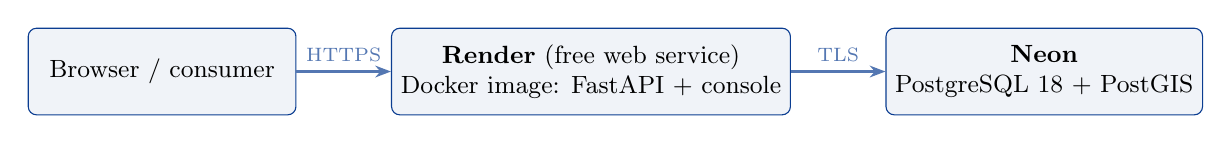
\begin{tikzpicture}[
  box/.style={draw=inha,fill=inha!6,rounded corners=3pt,align=center,font=\small,minimum height=1.1cm,minimum width=3.4cm},
  arr/.style={-{Stealth[length=2mm]},thick,inha!70}]
\node[box] (u) {Browser / consumer};
\node[box,right=1.2cm of u] (r) {\textbf{Render} (free web service)\\ Docker image: FastAPI + console};
\node[box,right=1.2cm of r] (n) {\textbf{Neon}\\ PostgreSQL 18 + PostGIS};
\draw[arr] (u) -- node[above,font=\scriptsize]{HTTPS} (r);
\draw[arr] (r) -- node[above,font=\scriptsize]{TLS} (n);
\end{tikzpicture}
\end{center}

\begin{itemize}
  \item \textbf{Image.} A two-stage \code{Dockerfile}: Node builds the console, then a
    Python 3.12 image installs the API and copies in \code{ui/dist}. Render builds it from
    the GitHub repository on its own servers (\code{render.yaml}). Every push to
    \code{main} redeploys automatically.
  \item \textbf{Database.} Neon runs PostgreSQL 18.7 with PostGIS 3.6.4. The schema
    and seed are loaded once, from a laptop, with the same \code{scripts/setup_db.py}
    pointed at Neon through \code{DATABASE_URL}. The container never builds the database,
    so a restart cannot touch the data.
  \item \textbf{Configuration.} A single \code{DATABASE_URL} (kept only in Render's
    environment, never committed) overrides the local \code{DB_*} settings. Because Neon
    closes idle connections, the pool checks each connection before handing it out.
  \item \textbf{Security.} Render generates a random \code{INGEST_API_TOKEN}, so the public
    demo does not accept the development token.
  \item \textbf{Health.} Render's health check calls \code{/health}, which returns 503
    without a database, so a wrong connection string fails the deploy instead of
    publishing a broken site.
\end{itemize}

The free tier sleeps after 15 idle minutes and needs about a minute to wake. The demo plan
is to open the site five minutes before presenting and keep the local build ready as a
fallback that needs no internet.

% =============================================================================
\section{Known limitations}\label{sec:limits}

The team states these limitations openly; none is hidden by the evidence.

\begin{itemize}
  \item \textbf{Synthetic data.} Only the bus stops and the AirKorea stations and readings
    are real. Everything else is generated and labelled as such (Section~\ref{sec:sources}).
  \item \textbf{DB3-3.} No official tourism visitor file is archived in the repository,
    so the totals cannot be reconciled with an official payload hash.
  \item \textbf{DB4-1.} The alert thresholds equal the AirKorea grade boundaries and are
    cited in \code{sql/05}, but a copy of the source document is not archived.
  \item \textbf{DB5-1.} The five facility coordinates are placeholders and have not been
    checked against the official facility file.
  \item \textbf{Registry levels.} The verification levels in \code{source_registry.csv}
    were taken from the assignment handbook and still need to be re-verified by the team.
  \item \textbf{Landmarks.} The 15 landmark coordinates are approximate.
  \item \textbf{Timings.} All timings come from one laptop and a modest data set. They
    show plan shapes and relative costs, not production capacity.
  \item \textbf{Docker Compose.} \code{compose.yaml} follows the assignment but was not
    run on the development machine. The \code{Dockerfile} is exercised by the deployment.
\end{itemize}

% =============================================================================
\section{Team roles and oral-defense preparation}\label{sec:team}

\subsection{Team and contributions}

The team has eight members in two groups, each with a leader. Every member contributed to
the domain listed below and can explain and run its part of the platform.

\begin{center}\small
\begin{tabularx}{\linewidth}{@{}p{3.6cm}p{1.6cm}p{1.3cm}X@{}}
\toprule
Member & Student ID & Role & Contribution \\
\midrule
Ibila Bekzat & 12235618 & Leader & DB1 Mobility and DB5 Safety \& Incident \\
Erkinbek Uulu Islam & 12240218 & Leader & DB3 Tourism, DB1 Mobility and DB4 Environment; the integrated web console (task runner, city map with time slider and live mode, ingestion forms, verification page) and its integration with the API \\
Madaminov Behzodbek & 12244958 & Member & DB2 Smart Building \\
Mahmudjonov Ulugbek & 12244978 & Member & DB2 Smart Building \\
Chomoev Bekbol & 12244955 & Member & DB3 Tourism \\
Karimov Dilshodbek & 12244940 & Member & DB4 Environment \\
Saidov Saidumar & 12244960 & Member & DB4 Environment \\
Ismoiljonov Boburjon & 12244956 & Member & DB5 Safety \& Incident \\
\bottomrule
\end{tabularx}
\end{center}

\subsection{Defense questions and answers}

\qa{Why must distances be computed on \texttt{geography} and not on
    \texttt{geometry(Point, 4326)}?}{%
    EPSG:4326 coordinates are angles in degrees. \cmd{ST_DWithin(geom, geom, 500)} would
    mean 500 degrees, and even small values are distorted because a degree of longitude
    shrinks with latitude (about 0.79 of a degree of latitude at Songdo). Casting to
    \code{geography} computes distances in metres on the WGS84 spheroid. This project met
    the problem directly: degree-based KNN ordering picked the wrong nearest station
    (Section~\ref{sec:cross}).}
\qa{How does the pipeline guarantee idempotency?}{%
    Each payload is hashed with SHA-256 over canonical JSON. A hash already staged for that
    source and table is reported as a duplicate. Domain tables have natural unique keys and
    are written with \cmd{ON CONFLICT}, so even concurrent identical requests store one row
    (12 parallel requests, 1 row).}
\qa{Why does \texttt{DISTINCT ON (vehicle\_id)} need \texttt{ORDER BY vehicle\_id,
    observed\_at DESC}?}{%
    \cmd{DISTINCT ON} keeps the first row of each group in sort order. The leading
    \code{vehicle_id} groups the rows, and \cmd{observed_at DESC} makes the first row the
    latest fix at or before $T$. Without the second key, the kept row would be arbitrary.}
\qa{What does the transaction in the pipeline protect?}{%
    The domain row, the audit entry and the staging status are written in one savepoint.
    Either all three exist or none does (CORE-2). A failing record rolls back only its own
    savepoint, so the rest of the batch still loads.}
\qa{How are concurrent incident transitions handled, and can they deadlock?}{%
    \code{transition_incident()} takes a row lock with \cmd{SELECT ... FOR UPDATE}. A
    second transaction on the same incident waits, then re-reads the new status and is
    rejected if its step is no longer legal (DB5-3-RACE). Each call locks exactly one
    incident row, so two calls cannot wait on each other in a cycle. A deadlock needs two
    transactions that each hold a lock the other wants. If one occurred elsewhere,
    PostgreSQL would detect it and abort one transaction with SQLSTATE 40P01; the client
    would retry.}
\qa{Why an exclusion constraint instead of a check in Python?}{%
    A check in application code reads, then writes. Two sessions can both read ``no
    overlap'' and both insert. The exclusion constraint is enforced by the database on a
    GiST index, so the second insert waits for the first and then fails (DB2-3-RACE).}
\qa{Why \texttt{REFRESH MATERIALIZED VIEW CONCURRENTLY}?}{%
    A plain refresh takes an exclusive lock, and readers wait. \code{CONCURRENTLY} builds
    the new contents beside the old and swaps the differences. It needs a unique index on
    the view, and it keeps the read API available during a refresh.}
\qa{Can data be updated or deleted?}{%
    Reference data can be corrected with \code{PATCH} and removed with \code{DELETE}, each with an
    audit entry holding the old and new values. A place or attraction is deleted only when nothing
    refers to it; an event is cancelled and a device retired instead, because deleting them would
    erase history. Measurements and GPS fixes are never edited in place: a correction is ingested as
    a new packet that replaces the value, and the audit log records it (Section~\ref{sec:edits}).}
\qa{How is ``the state of the city at time $T$'' reconstructed?}{%
    Nothing is overwritten. GPS fixes, status changes and device stays are all history
    rows. For any $T$ the query takes, per entity, the latest row at or before $T$
    (\cmd{DISTINCT ON} or \cmd{LATERAL ... ORDER BY ... LIMIT 1}), or the interval that
    contains $T$.}

% =============================================================================
\appendix
\section{Quickstart}\label{app:quickstart}

\begin{lstlisting}[language=bash]
# 1. once, as postgres (pgAdmin Query Tool)
#    CREATE ROLE songdo_admin LOGIN SUPERUSER PASSWORD 'songdo_local';
#    CREATE DATABASE songdo_urban_memory OWNER songdo_admin;

# 2. configure and install
cp .env.example .env                    # set DB_PORT (5432 or 5433)
python -m venv .venv && .venv\Scripts\activate
pip install -r requirements.txt

# 3. build the database (migrations 00-07, then the seed)
python fixtures/seed_fixtures.py 1000   # regenerates fixtures/seed_data.sql (deterministic)
python scripts/setup_db.py              # --reset rebuilds from zero

# 4. run
uvicorn api.main:app --port 8000        # http://127.0.0.1:8000/docs
python -m unittest tests/test_platform.py

# 5. console (optional; served by FastAPI after the build)
cd ui && npm install && npm run build && cd ..

# 6. consumers
python -m consumers.smart_mobility_adapter
python -m consumers.vip_building_env_client
python -m consumers.digital_twin_temporal_replay

# 7. evidence (about 3.5 minutes; never touches the working database)
python scripts/evidence.py
\end{lstlisting}

The first spatial query of the assignment's quickstart (places within 1,000 m of a point,
measured on \code{geography}) corresponds to task CORE-1 in the console and to
\cmd{GET /api/v1/core/places/nearby} in the API.

\section{Task catalogue}\label{app:tasks}

\begingroup\small
\begin{xltabular}{\linewidth}{@{}p{1.45cm}Xp{5.6cm}@{}}
\caption{All 36 runnable tasks (parameters in brackets).}\label{tab:tasks}\\
\toprule
ID & Title & Parameters \\
\midrule
\endfirsthead
\toprule
ID & Title & Parameters \\
\midrule
\endhead
\bottomrule
\endfoot
CORE-1 & Places near a point & lon, lat, radius\_m \\
CORE-2 & Source registry & -- \\
CORE-3 & Quarantined records & limit \\
CORE-4 & Audit ledger (latest events) & limit \\
DB1-1 & Ordered route sequence & route\_number, direction \\
DB1-2 & Trip execution and stop arrivals & trip\_id \\
DB1-3 & Historical position replay & as\_of \\
DB1-4 & Peak-hour lateness and gap analysis & route\_number, from\_time, to\_time, limit \\
DB1-5 & Smart Mobility telemetry: candidate stops & vehicle\_id, radius\_m, last\_n \\
DB2-1 & Building and address reconciliation & max\_distance\_m \\
DB2-2 & Space hierarchy and device registration & building\_id \\
DB2-3 & Device relocation history & device\_id, as\_of \\
DB2-4 & Missing heartbeat and fault detection & as\_of, silent\_minutes \\
DB2-5 & VIP facility state retrieval & building\_id, as\_of \\
DB3-1 & Attractions and accessibility metadata & wheelchair\_only, parking\_only \\
DB3-2 & Event management and schedule integrity & from\_date, to\_date \\
DB3-3 & Official statistics vs.\ synthetic samples & month \\
DB3-4 & Open attractions near transit & stop\_number, radius\_m, day\_of\_week, at\_time \\
DB3-5 & Temporal demand and crowd forecasting & event\_date, radius\_m, window\_min \\
DB4-1 & Station registration and unit standards & station \\
DB4-2 & Telemetry ingestion and quality flags & station, as\_of \\
DB4-3 & Fault handling and late arrivals & from\_time, to\_time, late\_minutes, only\_problems \\
DB4-4 & Hourly rollup and threshold alerts & station, type\_code, day \\
DB4-5 & Contextual air exposure service & lon, lat, as\_of \\
DB5-1 & Public safety facilities registration & responder \\
DB5-2 & Incident creation and severity triage & from\_time, to\_time, limit \\
DB5-3 & State machine transitions and drills & incident\_id \\
DB5-4 & Response time analytics by facility & from\_date, to\_date, include\_drills \\
DB5-4B & Incident hotspots (spatial clusters) & from\_date, to\_date, eps\_m, min\_points, limit \\
DB5-5 & Smart Mobility hazard avoidance & as\_of \\
X-1 & Attractions and events near transit stops & stop\_number, on\_date, limit \\
X-2 & Building devices with outdoor air context & building\_id \\
X-3 & Incidents impacting transit and air context & limit \\
X-4 & Place context cards (materialized view) & category \\
X-5 & Facility response statistics (materialized view) & from\_date, to\_date, include\_drills \\
X-6 & Materialized view freshness & -- \\
\end{xltabular}
\endgroup

\section{Evidence file index}\label{app:files}

\begin{center}\small
\begin{tabularx}{\linewidth}{@{}p{5.2cm}X@{}}
\toprule
File in \code{outputs/evidence/} & Content \\
\midrule
\code{README.md} & Summary report: gates, acceptance matrix, performance, API, console \\
\code{verification_summary.csv} & Gate checklist \\
\code{environment.txt} & Versions of every component and the git commit \\
\code{clean_build.log}, \code{schema_inventory.csv} & psql output of the clean build; object and row counts \\
\code{acceptance_matrix.csv} & Scenario acceptance checks \\
\code{test_results.txt} & Verbose unittest output \\
\code{backup_restore.log}, \code{backup_restore.csv} & Dump and restore commands; original vs.\ restored comparison \\
\code{performance.csv}, \code{explain_plans.md} & Timing and plan of every task; full \cmd{EXPLAIN ANALYZE} plans \\
\code{index_comparison.csv}, \code{scale_benchmark.csv} & Index vs.\ no index on the fixtures and on 1,000,000 rows \\
\code{api_contract.csv}, \code{api_latency.csv} & API cases and endpoint latency \\
\code{ui_task_coverage.csv}, \code{screenshots/} & Browser run of every task; 41 screenshots \\
\bottomrule
\end{tabularx}
\end{center}

\end{document}
